\documentclass[12pt]{article}

\usepackage{booktabs}% http://ctan.org/pkg/booktabs
\usepackage[utf8]{inputenc}
\usepackage{changepage}
\usepackage{pgfplots}
\usepackage{amssymb}
\usepackage{xcolor}
\usepackage{hyperref}
\usepackage{listings}
\usepackage[T1]{fontenc}
\usepackage[utf8]{inputenc}
\usepackage{adjustbox}
\usepackage{amsmath}
\usepackage{mathtools}
\usepackage{biblatex}
\lstset{
  language=Python,
  numbers=left,
  numberstyle=\tiny,
  stepnumber=1,
  numbersep=5pt,
  tabsize=4,
  basicstyle=\ttfamily,
  columns=fullflexible,
  keepspaces,
}
\hypersetup{
    colorlinks,
    citecolor=black,
    filecolor=black,
    linkcolor=black,
    urlcolor=black
}

% Set page size and margins
% Replace `letterpaper' with `a4paper' for UK/EU standard size
\usepackage[letterpaper,top=2cm,bottom=2cm,left=3cm,right=3cm,marginparwidth=1.75cm]{geometry}

% Useful packages
\usepackage{amsmath}
\usepackage{mathtools}
\usepackage{graphicx}

\title{Appunti di Algebra lineare e Geometria}
\date{A.A 2022-20}

\newenvironment{para}{\begin{adjustwidth}{13mm}{}}{\end{adjustwidth}}

\newcommand\tab[1][1cm]{\hspace*{#1}}

\newcommand{\tabitem}{\llap{\textbullet}}
\newcommand{\Hsquare}{%
\text{\fboxsep=-.2pt\fbox{\rule{0pt}{1ex}\rule{1ex}{0pt}}}%
}

\newtheorem{Definizione}{Definizione}[subsection]
\newtheorem{Lemma}{Lemma}[subsection]
\newtheorem{Teorema/Definizione}{Teorema/Definizione}[subsection]
\newtheorem{Corollario}{Corollario}[subsection]
\newtheorem{Teorema}{Teorema}[subsection]
\newtheorem{Proposizione}{Proposizione}[subsection]
\newtheorem{Notazione}{Notazione}[subsection]
\newtheorem{Commento}{Commento}[subsection]
\newtheorem{Dimostrazione}{Dimostrazione}[subsection]
\newtheorem{Osservazione}{Osservazione}[subsection]
\newtheorem{Nota}{Nota}[subsection]

\title{Linguaggi e computabilità}
\author{spitfire}
\date{November 2023}
\begin{document}

\begin{figure}
\centering

\includegraphics[width=0.35\textwidth]{images/Logo scienze bicocca.png}
\end{figure}

\vspace{10cm}
\date{A.A. 2023-2024}
\maketitle

\newpage

\tableofcontents
\newpage
\section{Concetti generali della teoria degli automi}
\begin{Definizione}[Alfabeto]
    Con alfabeto si intende un insieme non vuoto di simboli. Esso si indica con $\Sigma$ oppure $\Gamma$.
\end{Definizione}
\begin{Definizione}[Stringa]
    Con stringa si identifica una sequenza finita di simboli di un alfabeto. Una stringa, tuttavia, non può essere costruita su più alfabeti.
\end{Definizione}
\begin{Definizione}[Stringa vuota]
    Viene indicata con $\varepsilon$ (o $\lambda$) la stringa vuota. Essa è una sequenza formata da 0 simboli dell'alfabeto
\end{Definizione}
\begin{Definizione}[Lunghezza di una stringa]
    La lunghezza di una stringa a è il numero di caratteri da cui è composta. Essa si indica con $|a|$.
\end{Definizione}
\begin{Definizione}[Potenze di un alfabeto]
    Sia $\Sigma$ un alfabeto. Possiamo esprimere l'insieme di tutte le stringhe di una certa lunghezza k usando una notazione esponenziale. Definiamo quindi con $\Sigma^k$ come l'insieme delle stringhe di lunghezza k costruite a partire dall'alfabeto $\Sigma$. In particolare, abbiamo:
    $$\Sigma^0 = \{\varepsilon\}$$
    $$\Sigma^* = \Sigma^0 \cup \Sigma^1 \cup ... = \bigcup_{k \geq 0}^{+\infty} \Sigma^k$$
    $$\Sigma^+ = \Sigma^1 \cup \Sigma^2 \cup ... = \bigcup_{k = 1}^{+\infty} \Sigma^k = \Sigma^* \backslash \{\varepsilon\}$$
\end{Definizione}
\begin{Definizione}[Concatenazione di stringhe]
    Siano x e y delle stringhe. Allora la loro concatenazione xy è data facendo seguire ad una copia di x una copia di y. Essa si indica anche con il simbolo $\cdot$
\end{Definizione}
\begin{Osservazione}
    $|x \cdot y| = |x| + |y|$
\end{Osservazione}
\begin{Osservazione}
    $|x \cdot \varepsilon| = |\varepsilon \cdot x| = |x|$
\end{Osservazione}
\begin{Osservazione}
    $(\Sigma^*, \cdot)$ è un \textbf{monoide} libero con elemento neutro $\varepsilon$. Cioè è un semigruppo dotato di base per i suoi elementi.
\end{Osservazione}
\begin{Definizione}[Linguaggio]
Dato un alfabeto $\Sigma$, un linguaggio L su $\Sigma$ è un sottoinsieme di $\Sigma^*$: $L \subseteq \Sigma*$.
\end{Definizione}
\begin{Osservazione}
    Un linguaggio può contenere un numero infinito di stringhe. Per descrivere tali linguaggio si può usare questa notazione: $$L_A = \{x \in \Sigma^* | A(x) = Si\}$$
    Con A l'automa che riconosce se se una stringa in input fa parte del linguaggio o meno
\end{Osservazione}
\newpage
\begin{Definizione}[Mebership problem]
Dato $L \subseteq \Sigma^*$ e data una strina $x \in \Sigma^*$, $x \in L$?. Di solito il problema viene risolto o tramite il metodo dell'\textbf{automa} o oppure si utilizza una grammatica per il Linguaggio L; quindi $x \in L \Leftrightarrow$ x si può derivare dalle regole della grammatica. Il problema è analogo ad un \textbf{problema di decisione}; in particolare esso è un \textbf{problema di decisione universale}, poiché può essere rappresentato in molteplici modi.
\end{Definizione}
\section{Linguaggi e grammatiche}
\subsection{Linguaggi Context-Free}
I linguaggi Context-Free possono essere utilizzati per definire la \textbf{sintassi} dei linguaggi di programmazione e/o di rappresentazione (HTML, XML, ...). Essi hanno una \textbf{struttura ricorsiva} e hanno principalmente due regole di composizione:
\begin{enumerate}
    \item \textbf{Concatenazione}: Un linguaggi L è composto da due linguaggi, $L_1$ e $L_2$ concatenati l'uno dietro l'altro
    \item \textbf{Linguaggio contenuto in un altro}: L è un linguaggio che contiene un linguaggio $L_1$ contenuto all'interno delle stringhe di un altro linguaggio $L_2$.
\end{enumerate}
\subsection{Grammatiche e produzioni}
\begin{Definizione}
    Una Grammatica G è una quadrupla $G = (V, T, P, S)$ dove:
    \begin{itemize}
        \item $V$ = Insieme delle variabli
        \item $T$ = Insieme dei simboli terminali
        \item $P$ = Insieme delle regole di produzione
        \item $S$ = "Starting symbol" $\in V$
    \end{itemize}
    In particolare, le regole di produzione hanno questa sintassi: supponendo l'esistenza in V di una variabile $X$
    $$X \to Prod_1|Prod_2|...|Prod_n$$
    Mentre una particolare derivazione ha questa sintassi:
    $$X \Rightarrow Prod_1 \Rightarrow ...$$
\end{Definizione}
\begin{Osservazione}
    Il processo di derivazione \textbf{non è controllato}; cioè la \newline grammatica, applicando ogni combinazione delle regole di produzione, \textbf{produce ogni stringa possibile}
\end{Osservazione}
\begin{Osservazione}
    In ogni passo di derivazione, la grammatica pratica \textbf{al più una sostituzione}
\end{Osservazione}
\subsection{Tipi di Linguaggi e grammatiche}
Le grammatiche si differenziano fra loro per la struttura delle regole di produzione. \textbf{Noam Chomsky} teorizzò per primo la \textbf{gerarchia dei linguaggi}:
$$Tipo \; 0 \supseteq Tipo \; 1 \supseteq Tipo \; 2 \supseteq Tipo \; 3$$
I linguaggi quindi si dividono in 4 possibili tipi e si differenziano anche sulla struttura degli automi che accettano i linguaggi di un certo tipo rispetto ad un altro:
\begin{itemize}
    \item \textbf{Tipo 0: Linguaggi ricorsivamente enumerabili}: In questi linguaggi le regole di produzione possono essere solo del tipo $$\alpha \rightarrow \beta \; con \; \alpha, \beta \in (V \cup T)^*$$
    Gli automi che accettano questo tipo di linguaggi sono le \textbf{Macchine di Turing}
    \item \textbf{Tipo 1: Linguaggi contestuali o "dipendenti dal contesto"}: In questi linguaggi le regole di produzione sono del tipo: $$\alpha_1 A \alpha_2 \rightarrow \alpha_1 \beta \alpha_2 \; con \; \alpha_1,\alpha_2,\beta \in (V \cup T)^*, \beta \neq \varepsilon \; e \; A \in V$$
    $\alpha_1, \alpha_2$ sono il \textbf{contesto} della variabile A; cioè la sostituzione avviene solamente se A è tra $\alpha_1, \alpha_2$. Gli automi che accettano questi linguaggi sono le \textbf{Macchine di Turing che lavorano in spazio lineare}
    \item \textbf{Tipo 2: Linguaggi Context-Free o "liberi dal contesto"}: In questi linguaggi, le regole di produzione sono del tipo $$A \rightarrow \beta \; dove \; A \in V \; e \; \beta \in (V \cup T)^*$$
    Gli auotomi che accettano questi linguaggi sono gli \textbf{Automi a pila non deterministici}
    \begin{Osservazione}
        Le regole di tipo 2 sono un caso particolare delle regole di tipo 1
    \end{Osservazione}
    \item \textbf{Tipo 3: Linguaggi regolari}: Le regole di produzione di questi linguaggi sono del tipo:
    $$A \rightarrow aB \; oppure A \; \rightarrow a \; dove A,B \in V \; e \; a \in T$$
    Gli automi che accettano questi linguaggi sono gli \textbf{Automi a stati finiti deterministici, non-deterministici e non-deterministici con $\varepsilon$-transizioni}
\end{itemize}
\begin{Proposizione}
Le \textbf{variabili} sono anche dette \textbf{categorie sintattiche}; se vi sono 2 regole del tipo: $$A \to B$$ $$B \to C | D |...$$
Con B che non permette di tornare ad A; allora B può essere considerata come una \textbf{sottogrammatica}
\end{Proposizione}
\subsection{Metodo dell'inferenza ricorsiva}
Un altro metodo per derivare una stringa da una grammatica è quello dell'\textbf{inferenza ricosrsiva}:
\begin{enumerate}
    \item Si assegna ad ogni regola di produzione un numero
    \item Si costruisce una tabella con campi rispettivamente n° passo, stringa derivata, variabile usata, n° della produzione usata, stringhe pregresse usate (identificate con il n° di passo)
    \item si riempe la tabella derivando la stringa deisderata
\end{enumerate}
\begin{Osservazione}
    Utilizzare direttamente una derivazione o usare il metodo dell \textbf{inferenza ricorsiva} è equivalente
\end{Osservazione}
\subsection{Derivazioni}
\begin{Definizione}[$\Rightarrow$]
Sia $G = (V, T, P, S)$ una grammatica libera dal contesto (CFG da questo momento in poi). Sia $\alpha A \beta$ t.c. $\alpha \in (V \cup T)^*, A \in V$. Sia $A \to \gamma$ una regola di produzine con $\gamma \in (V \cup T)^*$. Allora scriviamo: $\alpha A \beta \Rightarrow \alpha \gamma \beta$.
\end{Definizione}
\begin{Definizione}[$\Rightarrow^*$]
    La definizione di derivazione in "zero o più passi" è induttiva:
    \begin{itemize}
        \item \textbf{Base}: $\forall \alpha \in (V \cup T)^*, \alpha \Rightarrow^* \alpha$
        \item \textbf{Passo induttivo}: Se $\alpha \Rightarrow^* \beta$ e $\beta \Rightarrow \gamma$ allora $\alpha \Rightarrow^* \gamma$
    \end{itemize}
\end{Definizione}
\begin{Definizione}[$\Rightarrow^*$ alternativa]
    $\alpha \Rightarrow^* \beta$ se $\exists \gamma_1, \gamma_2, ..., \gamma_n$, con $n \geq 1$ t.c. \newline $\alpha = \gamma_1, \beta = \gamma_2$ e $\forall i = 1,2,...,n-1$ vale che $\gamma_i \Rightarrow \gamma_{i+1}$
\end{Definizione}
\begin{Notazione}
Se si opera su una grammatica G oppure vi è ambiguità, allora si scrive $\Rightarrow_{G}^*$
\end{Notazione}

\begin{Definizione}[$\Rightarrow_{lm}$]
Una derivazione è "left-most" quando si sostituisce \textbf{sempre} la variabile più a sinistra
\end{Definizione}
\begin{Definizione}[$\Rightarrow_{rm}$]
Una derivazione è "right-most" quando si sostituisce \textbf{sempre} la variabile più a destra
\end{Definizione}
\begin{Teorema}
$A \Rightarrow^* w$ (con $A\in V$ e $w \in (V \cup T)^*$) $\Leftrightarrow$ si può derivare $A \Rightarrow_{lm}^* w$ e $A \Rightarrow_{rm}^* w$
\end{Teorema}
\subsection{Linguaggio generato da una CFG}
Data una CFG $G = (V, T, P, S)$, il linguaggio generato da G è $$L(G) = \{w \in T^* | S \Rightarrow^* w \}$$
\begin{Definizione}[Forma sentenziale]
    Data una $G = (V, T, P, S)$, una forma sentenziale è una stringa $\alpha \in (V \cup T)^*$ t.c. $S \Rightarrow^* \alpha$
\end{Definizione}
\newpage
\subsection{Linguaggi di tipo 1: Linguaggi contestuali}
Vediamo alcuni esempi di linguaggi contestuali: \newline
\textbf{1° Esempio}
$$L = \{a^n b^n c^n | n \geq 1 \}$$
$$G = \bigl\{\{S, B, C, X\}, \{a,b,c\}, P, S \bigl\}$$
\textbf{P}:
\begin{enumerate}
    \item $S \to aSBC$
    \item $S \to aBC$
    \item $CB \to XB$
    \item $XB \to XC$
    \item $XC \to BC$
    \item $aB \to ab$
    \item $bB \to bb$
    \item $bC \to bc$
    \item $cC \to cc$
\end{enumerate}
Supponiamo di avere (segnamo in \textbf{grassetto} il contesto di ogni variabile):
$$...C\textbf{B}...\Rightarrow_3 \textbf{X}B \Rightarrow_4 X\textbf{C} \Rightarrow_5 BC$$
cioè $CB \Rightarrow^* BC$
Per ottenere quindi una qualsiasi stringa, in generale:
$$S \Rightarrow_1^{n-1} a^{n-1}S(BC)^{n-1} \Rightarrow_2 a^n(BC)^n \Rightarrow_{3,4,5}^{n(n+1)/2}a^n b^n c^n \Rightarrow_6 a^bB^{n-1}C^n \Rightarrow_7^{n-1} a^n b^n C^n$$
$$\Rightarrow_8 a^n b^n cC^{n-1} \Rightarrow_9^{n-1} a^n b^n c^n$$
Perchè $\Rightarrow_{3,4,5}$ deve essere applicato $n(n+1)/2$ volte?
\begin{Dimostrazione}
Procediamo per induzione su n:
\begin{itemize}
    \item \textbf{Base (n=1)} $BC \Rightarrow^{1(1-1)/2} BC$
    \item \textbf{Passo induttivo}: Supponiamo $(BN)^n \Rightarrow_{3,4,5}^{n(n+1)/2} B^n C^n$ vero e dimostriamo che vale anche per n+1:
    $$(BC)^{n+1} = (BC)^n BC \Rightarrow_{3,4,5}^{n(n-1)/2} B^n C^n BC \Rightarrow_{3,4,5}^{n} B^{n+1} C^{n+1}$$
    Il numero di applicazioni è quindi $n(n-1)/2 + n = n(n+1)/2 $
\end{itemize}
\begin{flushright}
    $\square$
\end{flushright}
\end{Dimostrazione}
\textbf{2° esempio}:
$$L = \{a^n b^m c^n d^m | n, m \geq 1\}$$
Il linguaggio è evidentemente di tipo 1, visto che presenta un "accavallamento" tra n e m che non permetterebbe di esprimerne una grammatica seguendo solo regole di tipo 2
\newpage
\subsection{Alberi sintattici}
Un \textbf{albero sintattico} è una struttura ad albero che rappresenta come una certa sequenza di caratteri è stata ottenuta; quest'ultima è indicata come il \textbf{prodotto dell'albero}.
\begin{center}
    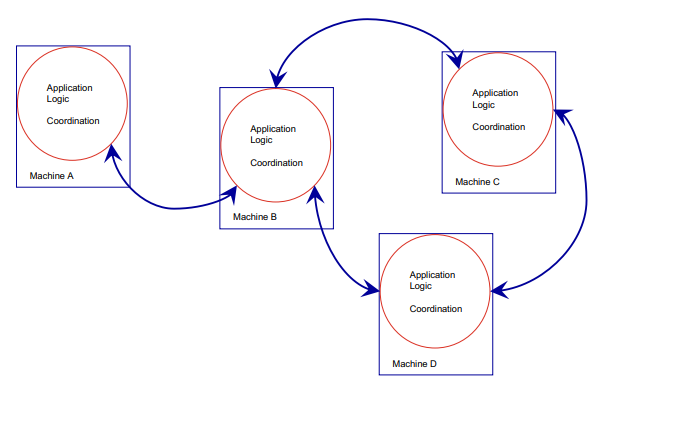
\includegraphics[width = 0.40\textwidth]{images/1.PNG}
\end{center}
\begin{Definizione}[Albero sintattico]
    Data una grammatica $G = (V, T, P, S)$, allora un albero sintattico per G è tale che:
    \begin{itemize}
        \item Ogni nodo interno è etichettato da una variabile
        \item Ogni foglia è etichettata da una variabile, da un simbolo terminale oppure da $\varepsilon$. Se una foglia è etichettata da $\varepsilon$, deve essere l'unico figlio del suo genitore
        \item Se un nodo interno è eitchettato da A e i suoi figli sono etichettati, a partire da sinistra, con $x_1, x_2, ..., x_k$, allora $A \to x_1x_2...x_k$ è una regola di produzione di P.
        \item Gli alberi sintattici sono \textbf{ordinati}
    \end{itemize}
\end{Definizione}
\begin{Osservazione}
    Se un sottoalbero si trova a sinistra/destra di un altro sottoalbero, allora la formula indicata da esso si trova a sinistra/destra della formula indicata dall'altro sottoalbero
\end{Osservazione}
\begin{Teorema}
    Data una CFG G e un linguaggio A, i seguenti enunciati si equivalgono:
    \begin{itemize}
        \item L'inferenza ricorsiva stabilisce che la stringa terminale w è nel linguaggio delal variabile A $\Leftrightarrow$
        \item $A \Rightarrow^* w \Leftrightarrow$
        \item $A \Rightarrow_{lm}^* w \Leftrightarrow$ 
        \item $A \Rightarrow_{rm}^* w \Leftrightarrow$
        \item Esiste un albero sintattico con radice A e prodotto w.
    \end{itemize}    
\end{Teorema}
\begin{Dimostrazione}
    Questa equivalenza è dimostrabile secondo il seguente schema:
    \begin{center}
        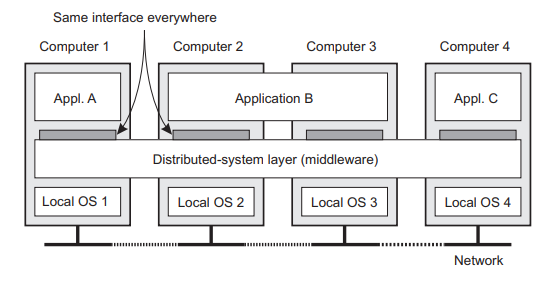
\includegraphics[width = 0.60\textwidth]{images/2.PNG}
    \end{center}
    Ogni arco del grafo denota un teorema secondo il quale, se w soddisfa la condizione nella \textbf{coda dell'arco}, la soddisfa anche nella \textbf{testa dell'arco}. Per esempio, se si deduce che w è nel linguaggio per \textbf{inferenza ricorsiva}, allora esiste anche un albero sintattico T con radice A e prodotto w.
\end{Dimostrazione}
\subsection{Ambiguità}
Una stringa w di terminali può essere \textbf{ambigua}; cioe può avere \textbf{più di un albero sintattico} da cui è possibile derivarla. L'ugaglianza degli alberi quindi crea problemi ad un potenziale \textbf{parser sintattico} per il linguaggio. L'ideale sarebbe quindi che le grammatiche \textbf{non fossero ambigue}, tuttavia ci sono delle \textbf{cattive notizie}:
\begin{itemize}
    \item In generale, non esiste un algoritmo che determina se una CFG G è ambigua o meno
    \item Data una CFG G che \textbf{sappiamo} essere ambigua, non esiste un algoritmo che ci consente di trasformarla
    in una CFG G' \textbf{non ambigua}
    \item Esistono \textbf{linguaggi ineritamente ambigui}, cioè per i quali non esiste nessuna CFG \textbf{non} ambigua.
\end{itemize}\subsubsection{Ambiguità e left-most derivation}
\begin{Teorema}
    $\forall CFG \; G = (V, T, P, S)$ e $\forall w \in T^*$, abbiamo che w ha 2 alberi sintattici distinti $\Leftrightarrow$ ha 2 derivazioni sinistre distinte.
\end{Teorema}
\subsubsection{Ambiguità inerente}
\begin{Definizione}[Linguaggio inerentemente ambiguo]
Un linguaggio si dice inerentemente ambiguo se esso \textbf{non ammette grammatiche non ambigue}; cioè tutte le sue grammatiche sono ambigue
\end{Definizione}
\newpage
\subsection{Grammatiche regolari}
\begin{Definizione}[Grammatica regolare]
Sia $G = (V, T, P, S)$. Se:
\begin{enumerate}
    \item $\varepsilon$ può comparire solo nella regola $S \to \varepsilon$, dove S è lo "starting symbol"
    \item Le regole di produzione P sono \textbf{tutte} lineari a destra oppure \textbf{tutte} lineari a sinistra; cioè se
    \begin{itemize}
        \item \textbf{lineare a dx}: $A \to aB$ oppure $A \to a$ dove $A,B \in V$ e $a \in T$
        \item \textbf{lineare a sx}: $A \to Ba$ oppure $A \to a$ dove $A,B \in V$ e $a \in T$
    \end{itemize}
\end{enumerate}
Allora la grammatica è \textbf{regoalre}
\end{Definizione}
\begin{Proposizione}
    Usando solo le regoli lineari a sx/dx, ottengo \textbf{tutti i linguaggi regolari}. In particolare, posso trasformare un linguaggio che usa una delle 2 nell'alternativa
\end{Proposizione}
\subsection{Operazioni su linguaggi}
Vi sono principalmente tre operazioni possibili sui linguaggi:
\begin{itemize}
    \item \textbf{Unione}: Dati due linguaggi L e M su un certo alfabeto $\Sigma$, allora la loro unione $L \cup M$ è l'insieme delle stringhe appartenenti ad L e M, prese una sola volta
    \item \textbf{Concatenazione}: Dati L e M, abbiamo che la loro concatenazione $LM = \{w=w_1w_2|w_1 \in L, w_2 \in M\}$. In particolare, l'insieme LM contiene tutte le stringhe che si possono formare prendendo una qualsiasi stringa di L e concatenandola con una qualsiasi stringa di M. La cardinalità di LM è $|LM| = |L| \cdot |M|$; inoltre $|L \cup M| \leq |L| + |M|$
    \item \textbf{Chiusura (o "star") di Kleene}: La chiusura di Kleene di un linguaggio L viene indicata con $L^*$ e rappresenta l'insieme delle stringhe che possono essere formate prendendo il linguaggio L e \textbf{concatenandolo} con se stesso infinite volte. Formalmente quindi:
    $$L^* = \bigcup_{i=0}^{+\infty}L^i$$
    $$L^i = \underbrace{L \cdot L \cdot L \cdot L ... \cdot L}_{i-volte}$$
    In particolare: $$L^1 = L$$ $$L^0 = \{\varepsilon\}$$
    \begin{Osservazione}
        Se $|L| = q$, allora $|L^i| = q^i$
    \end{Osservazione}
    \begin{Proposizione}
        La stella di kleene è definibile anche su linguaggi infiniti
    \end{Proposizione}
    Vi sono ancora due casi particolari:
    $$L = \emptyset \Rightarrow L^0 = \emptyset^0 = \{\varepsilon\} \; mentre \; L^i = \underbrace{\emptyset \cdot \emptyset \cdot ... \cdot \emptyset}_{i-volte} = \emptyset$$
    $$L = \{\varepsilon\} \Rightarrow L^0 = \{\varepsilon\}^0 = \{\varepsilon\} mentre \; L^i = \underbrace{\{\varepsilon\} \cdot \{\varepsilon\} \cdot ... \cdot \{\varepsilon\}}_{i-volte} = \{\varepsilon\}$$
    Quanto vale quindi la stella di kleene in questi due casi?
    $$L = \emptyset \Rightarrow L^* = \{\varepsilon\}$$
    $$L = \{\varepsilon\} \Rightarrow L^* = \{\varepsilon\}$$
    Essi sono gli unici 2 casi in cui la chiusura di Kleene è un insieme finito.
\end{itemize}
\subsection{Espressioni Regolari (ER)}
Le espressioni regolari si usano per rappresentare (in termini tecnici, \textbf{denotare}) i linguaggi regolari.
\begin{Definizione}[Espressioni regolari]
La definizione procede per induzione:
\begin{itemize}
    \item \textbf{Base}: $\varepsilon$ e $\emptyset$ sono \textbf{espressioni regolari}. Questi due simboli, tuttavia non denotano la stringa vuota o l'insieme vuoto, ma \textbf{i linguaggi denotati dall'insieme vuoto e da $\varepsilon$}, i quali sono $$L(\varepsilon) = \{\varepsilon\}$$ $$L(\emptyset) = \emptyset$$
    Se $a \in \Sigma$ (vogliamo denotare un linguaggio $L \subseteq \Sigma^*$, cioè un linguaggio costituito con i simboli di $\Sigma$) allora \textbf{a} è un espressione regolare che denota il linguaggio $$L(\textbf{a}) = \{a\}$$ 
    Le variabili che rappresentano i linguaggi (es. L) \textbf{sono espressioni regolari}.
    \item \textbf{Passo induttivo}
    \begin{enumerate}
        \item \textbf{Unione}: Se E ed F sono espressioni regolari, allora E + F è un espressione regolare. $$L(E+F) = L(E) \cup L(F)$$
        \item \textbf{Concatenazione}: Se E e F sono espressioni regolari, allora EF è un espressione regolare: $$L(EF) = L(E)L(F)$$
        \item \textbf{Chiusura}: Se E è un espressione regolare, allora $E^*$ è una espressione regolare: $$L(E^*) = (L(E))^*$$
        \item \textbf{Parentesi}: Se E è un espressione regolare, allora (E) è un espressione regolare $$L((E)) = L(E)$$
    \end{enumerate}
\end{itemize}
\end{Definizione}
\newpage
\subsubsection{Proprietà algebriche delle ER}
\begin{itemize}
    \item * si applica alla \textbf{più piccola sequenza di simboli a sinistra ben formata}.
    \item \textbf{Concatenazione}: Essa ha le seguenti proprietà:
    \begin{itemize}
        \item \textbf{Associativa}: $E \cdot (G \cdot F) = (E \cdot G) \cdot F = E \cdot G \cdot F$
        \item \textbf{Non} è commutativa: $EF \neq FE$
    \end{itemize}
    \item \textbf{Unione}: Essa ha le seguenti proprietà:
    \begin{itemize}
        \item \textbf{Associativa}: $E+(F+G) = (E+F)+G = E+F+G$
        \item \textbf{Commutativa}: $E+F = F+E$
    \end{itemize}
    \item $\emptyset$ è \textbf{l'identità} per l'unione: $\emptyset + L = L + \emptyset = L$
    \item $\varepsilon$ è \textbf{l'identità} per la concatenazione: $\varepsilon \cdot L = L \cdot \varepsilon = L$
    \item $\emptyset$ è \textbf{annichilatore} per la concatenazione: $\emptyset \cdot L = \emptyset$
    \item \textbf{Distributività sinistra della concatenazione sull'unione}: $$L(M+N) = LM + LN$$
    \item \textbf{Distributività destra della concatenazione sull'unione}: $$(M+N)L = ML + NL$$
    \item \textbf{Idempotenza dell'unione}: $L + L = L$
\end{itemize}
\section{Automi a stati finiti}
Vi sono 3 forme principali di automa a stati finiti:
\begin{itemize}
    \item Automi a stati finiti \textbf{deterministici} (DFA)
    \item Automi a stati finiti \textbf{non deterministici} (NFA)
    \item Automi a stati finiti \textbf{non deterministici con $\varepsilon$-transizioni}($\varepsilon$-NFA)
\end{itemize}
Tutti questi automi accettano \textbf{tutti e soli} i linguaggi regolari. Cioè: dato un linguaggio regolare L, esiste un automa a stati finiti $A_L$ che accetta ogni sua stringa.
\subsection{Automi a stati finiti deterministici (DFA)}
\begin{Definizione}[Automa a stati finiti deterministico (DFA)]
    Un DFA A è una quintupla: $$A = (Q, \Sigma, \delta, q_0, F)$$
    Dove:
    \begin{itemize}
        \item Q è l'insieme finito e non vuoto degli stati
        \item $\Sigma$ è l'alfabeto dei simboli in ingresso
        \item $\delta$ è la funzione di transizione degli stati
        \item $q_0 \in Q$ è lo stato iniziale
        \item $F \subseteq Q$ è l'insieme degli stati finali (o accettanti)
    \end{itemize}
\end{Definizione}
\begin{Definizione}[Funzione di transizione per DFA]
La funzione di transizione $\delta$ è definita come segue:
$$\delta: Q \times \Sigma \to Q$$
La funzione \textbf{deve essere totale}. In particolare, se $|Q| = n$ e $|\Sigma| = m$, allora il numero degli elementi di $\delta$ è $n \cdot m$.
\end{Definizione}
\subsubsection{Tabella di transizione}
Una tabella di transizione è una modalità di rappresentazione della funzione $\delta$. Le righe della tabella corrispondono agli stati, le colonne agli input. La voce all’incrocio della riga corrispondente allo stato q e della colonna corrispondente all’input a è lo stato $\delta(q, a)$
\begin{center}
    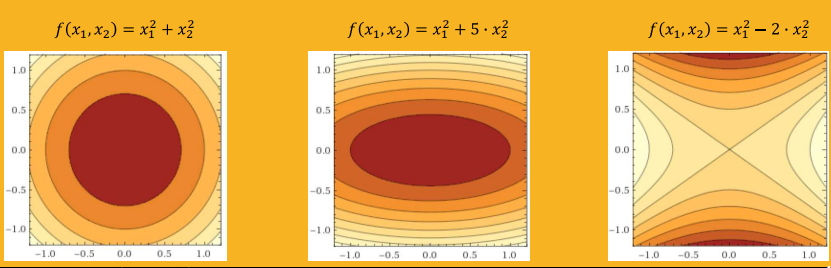
\includegraphics[width = 0.25\textwidth]{images/3.PNG}
\end{center}
In particolare, si indica con una $\to$ lo stato iniziale; mentre con un * gli stati finali.
\subsubsection{Diagramma di transizione}
Per un DFA, un diagramma di transizione è composto nel seguente modo:
\begin{itemize}
    \item Per ogni stato in Q esiste un \textbf{nodo}
    \item Per ogni stato q in Q e ogni simbolo di input $a \in \Sigma$, sia $\delta(q, a) = p$. Allora il grafo ha un arco dal nodo q al nodo p etichettato con a. Se esistono più simboli di input che portano da q a p, allora l'arco può essere etichettato dalla lista di tali simboli
    \item Una freccia etichettata \textbf{START} nello stato iniziale $q_0$. Tale freccia non proviene da nessuno nodo
    \item I nodi corrispondenti agli stati finali sono segnati con un doppio circolo.
\end{itemize}
\begin{center}
    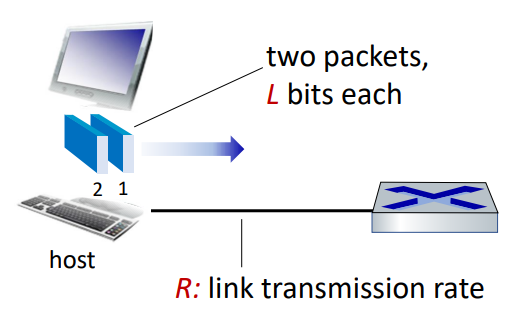
\includegraphics[width = 0.55\textwidth]{images/4.PNG}
\end{center}
\subsection{Funzione $\hat{\delta}$ per DFA}
Precisiamo la nozione di \textbf{linguaggio di un DFA}. Per farlo, dobbiamo quindi estendere la definizone di $\delta$ per adattarla a quando partiamo da uno stato q ed effettuiamo una serie di input; chiamiamo questa funzione estesa $\hat{\delta}$:
$$\hat{\delta}: Q \times \Sigma^* \to Q$$
\begin{Definizione}[$\hat{\delta}$]
La definizione procede per induzione:
\begin{itemize}
    \item \textbf{Base}: Se $|w| = 0$, allora $\hat{\delta}(q,w) = \hat{\delta}(q, \varepsilon) = q$
    \item  \textbf{Passo induttivo}: Se $|w| > 0$, allora w = ax, dove $a \in \Sigma$ e $x \in \Sigma^*$.
    Allora $\hat{\delta}(q, w) = \hat{\delta}(q, ax) = \hat{\delta}(\delta(q,a),x)$
\end{itemize}
\end{Definizione}
\begin{Definizione}[$\hat{\delta}$ alternativa]
La definizione procede per induzione:
\begin{itemize}
    \item \textbf{Base}: Se $|w| = 0$, allora $\hat{\delta}(q,w) = \hat{\delta}(q, \varepsilon) = q$
    \item  \textbf{Passo induttivo}: Se $|w| > 0$, allora w = xa, dove $a \in \Sigma$ e $x \in \Sigma^*$.
    Allora $\hat{\delta}(q, w) = \hat{\delta}(q, xa) = \delta(\hat{\delta}(q,x),a)$
\end{itemize}
\end{Definizione}
\subsection{Linguaggio accettato da un DFA}
\begin{Definizione}[Linguaggio accettato da un DFA]
    Il linguaggio accettato da un DFA A è definito come:
    $$L(A) = \{w \in \Sigma^* | \hat{\delta}(q_0, w) \in F \}$$
\end{Definizione}
\subsection{Automa a stati finiti non determinisstico (NFA)}
\begin{Definizione}[Automa a stati finiti non determinisstico (NFA)]
Un NFA è una quintupla $$N = (Q, \Sigma, \delta, q_0, F)$$
dove:
\begin{itemize}
        \item Q è l'insieme finito e non vuoto degli stati
        \item $\Sigma$ è l'alfabeto dei simboli in ingresso
        \item $\delta$ è la funzione di transizione degli stati
        \item $q_0 \in Q$ è lo stato iniziale
        \item $F \subseteq Q$ è l'insieme degli stati finali (o accettanti)
    \end{itemize}
\end{Definizione}
\begin{Definizione}[Funzione di transizione per NFA]
La funzione di transizione $\delta$ per NFA è definita come:
$$\delta: Q \times \Sigma \to 2^Q$$
Con $2^Q$ l'insieme delle parti di Q. In particolare, se $|Q| = n$ allora $|2^Q| = 2^{|Q|}$. La funzione delta \textbf{può anche non essere totale}.
\end{Definizione}
\subsubsection{Tabella degli stati per un NFA}
\begin{center}
    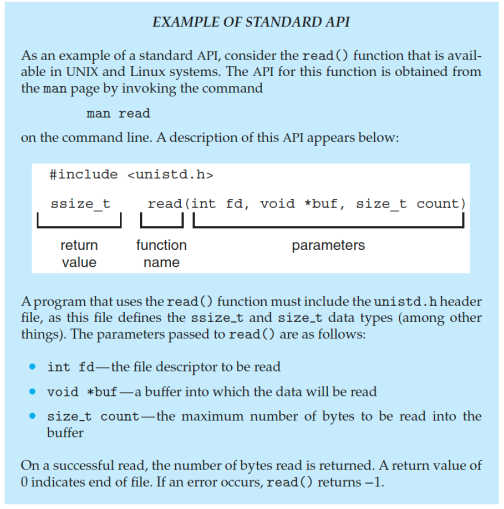
\includegraphics[width = 0.35\textwidth]{images/5.PNG}
\end{center}
La differenza sostanziale con la tabella per DFA è la funzione delta \textbf{ritorna un insieme di stati in cui l'NFA potrebbe transitare}.
\begin{Osservazione}
    Anche con un solo stato, l'output di $\delta$ per un NFA è sempre un insieme di stati
\end{Osservazione}
\begin{Osservazione}
    Ogni DFA può essere visto come caso particolare di NFA
\end{Osservazione}
\subsubsection{Interpretazione della computazione di un NFA}
\begin{center}
    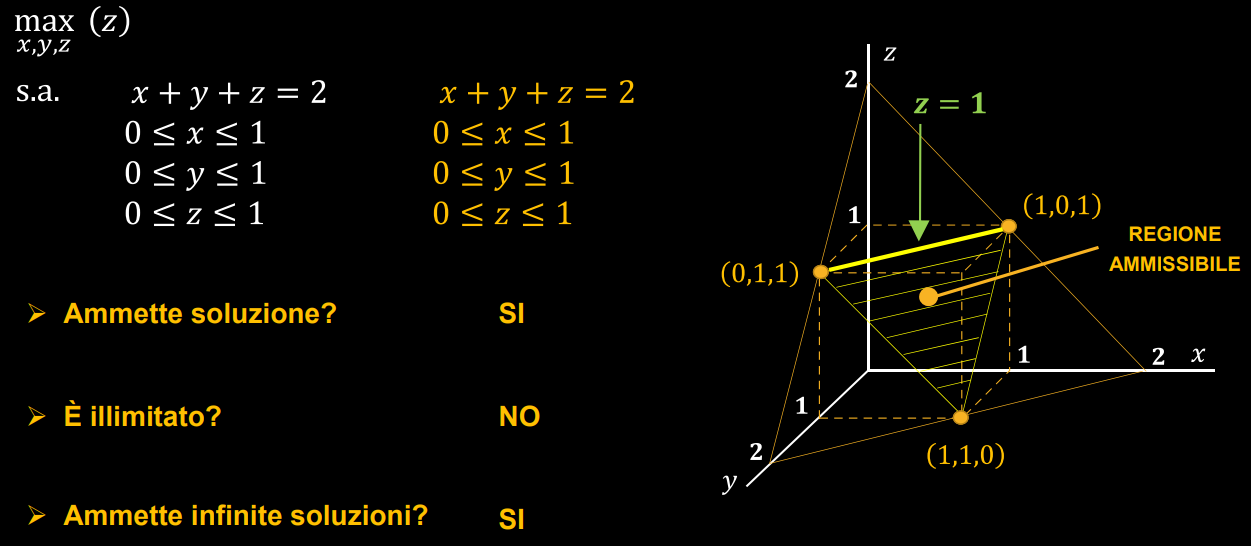
\includegraphics[width = 0.55\textwidth]{images/6.PNG}
\end{center}
Si può immaginare la computazione dell'NFA come una serie di \textbf{"processi paralleli"}: Partendo dallo stato iniziale, viene letto il primo carattere, l'automa può passare in una moltitudine di stati; immaginiamo quindi che facce \textbf{entrambe le cose contemporaneamente}; un processo quindi \textbf{"muore"} quando viene letto un carattere ma la funzione di transizione non è definita per quella particolare coppia Stato-Valore. La stringa è accetatta se almeno un processo è arrivato ad uno stato accettante.
\subsection{Linguaggio definito da un NFA}
$$L(N) = \{w \in \Sigma^* | \hat{\delta}_n(q_o, w) \cap F \neq \emptyset\}$$
Tuttavia, come fa un NFA a capire quale strada intraprendere o se ha finito la computazione? L'automa NFA può chiedere ad un \textbf{oracolo}, il quale "prevede il futuro" e sa qual'è il percorso corretto. Si può simulare questo oracolo? Per gli NFA, esso è simulabile tramie un \textbf{DFA} che accetta lo stesso linguaggio dell'NFA. Un problema però, se $|Q| = n$, allora $|2^Q| = 2^{|Q|} = 2^n$; poiché il DFA scandisce il diagramma dell'NFA "a blocchi" (ogni stato del DFA è un insieme di stati dell'NFA), c'è il rischio che si abbia un esplosione nel numero di stati da rappresentare
\subsection{$\hat{\delta}$ per NFA}
\begin{Definizione}[$\hat{\delta}$]
La definizione procede per induzione:
\begin{itemize}
    \item \textbf{Base}: Se $|w| = 0$, allora $\hat{\delta}(q,w) = \hat{\delta}(q, \varepsilon) = \{q\}$
    \item  \textbf{Passo induttivo}: Se $|w| > 0$, allora $w = ax$ con $a \in \Sigma$ e $w \in \Sigma^*$:
    $$\delta(q, a) = \{p_1, p_2, ..., p_k\}$$
    $$\hat{\delta}(q_i, w) = \bigcup_{i=1}^k \hat{\delta}(p_i, x) = \{R_1, ..., R_K\}$$
\end{itemize}
\end{Definizione}
\begin{Definizione}[$\hat{\delta}$ alternativa]
La definizione procede per induzione:
\begin{itemize}
    \item \textbf{Base}: Se $|w| = 0$, allora $\hat{\delta}(q,w) = \hat{\delta}(q, \varepsilon) = \{q\}$
    \item  \textbf{Passo induttivo}: Se $|w| > 0$, allora $w = xa$ con $a \in \Sigma$ e $w \in \Sigma^*$:
    $$\delta(q, x) = \{p_1, p_2, ..., p_k\}$$
    $$\hat{\delta}(q_i, w) = \bigcup_{i=1}^k \delta(p_i, a) = \{R_1, ..., R_K\}$$
\end{itemize}
\end{Definizione}
\subsection{Algoritmo di conversione NFA a DFA equivalente}
Per costruire il DFA $D = (Q_D, \Sigma, \delta_D \{q_s\}, F_D)$ a partire dall'NFA $N = (Q_N, \Sigma, \delta_N, q_0, F_N\}$ t.c $L(N) = L(D)$ partiamo dalle seguenti definizioni e adottiamo una tecnica chiamata "\textbf{costruzione per sottoinsiemi}":
\begin{itemize}
    \item $Q_D$ è l'insieme potenza di $Q_N$; quindi $Q_D = 2^{Q_N}$. Seppur la cardinalità di $|2^{Q_N}| = 2^{|Q_N|}$, non sempre si riescon a raggiungere tutti gli stati; quindi nel DFA gli stati potrebbero essere anche minori di $2^{|Q_N|}$
    \item $F_D = \{S \subseteq Q_N | S \cap F_N \neq \emptyset\}$, cioè $F_D$ è formato da tutti i sottoinsiemi di $Q_N$ che contengono almeno uno stato accettante
    \item Per ogni $S \subseteq Q_N$ e per ogni simbolo di input $a \in \Sigma$:
    $$\delta_D = \bigcup_{p \in S}\delta_N(p, a)$$
    Cioè, per computare $\delta_D(S, a)$ consideriamo tutti gli stati di S, rileviamo in quali insiemi di stati va a finire l'automa partendo da p e leggendo a e infine prendiamo l'unione di tutti questi sottoinsiemi.
\end{itemize}
\begin{center}
    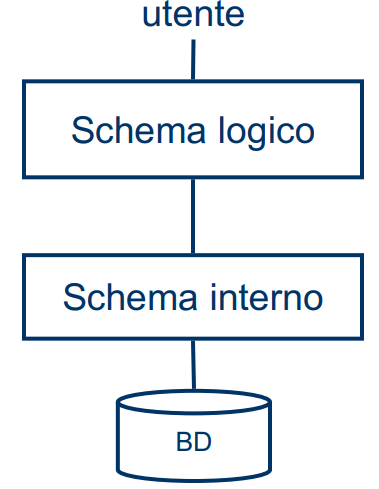
\includegraphics[width = 0.55\textwidth]{images/7.PNG}
\end{center}
Nominiamo infine ogni stato con una lettera e costruiamo il DFA equivalente.
\begin{Nota}
    Ogni transizione che porta all'insieme vuoto risulta in un \textbf{nodo pozzo}
\end{Nota}
\subsection{$\varepsilon$-NFA}
Gli $\varepsilon$-NFA sono particolari tipi di NFA che presentano le "$\varepsilon$-transizioni", cioè transizioni ad altri stati che \textbf{non comportano il consumo di un simbolo}. Quando una \newline $\varepsilon$-transizione viene eseguita dall'automa, si dice che esso ha fatto una $\varepsilon$-mossa
\begin{Definizione}[$\varepsilon$-NFA]
Un $\varepsilon$-NFA è una quintupla $$E = (Q, \Sigma, \delta, q_0, F)$$
Dove:
\begin{itemize}
        \item Q è l'insieme finito e non vuoto degli stati
        \item $\Sigma$ è l'alfabeto dei simboli in ingresso
        \item $\delta$ è la funzione di transizione degli stati
        \item $q_0 \in Q$ è lo stato iniziale
        \item $F \subseteq Q$ è l'insieme degli stati finali (o accettanti)
    \end{itemize}
\end{Definizione}
\begin{Definizione}[Funzione di transizione per $\varepsilon$-NFA]
La funzione di transizione $\delta$ per $\varepsilon$-NFA è definita nel seguente modo:
$$\delta: Q \times (\Sigma \cup \{\varepsilon\}) \to 2^Q$$
\end{Definizione}
\subsection{Eclose}
Sia $q \in Q$. Allora $Eclose(q)$ è \textbf{l'insieme} degli stati raggiungibili tramite $\varepsilon$-mosse (o 0 mosse). Essa è quindi una funzione definita come segue:
$$Eclose: Q \to 2^Q$$
\begin{Definizione}
La definizione procede per induzione:
\begin{itemize}
    \item \textbf{Base}: $q \in Eclose(q)$
    \item \textbf{Passo induttivo}: Se $p \in Eclose(q)$ ed esiste una transizione che porta da p ad r tramite una $\varepsilon$-mossa, allora $r \in Eclose(q)$
\end{itemize}
\end{Definizione}
\subsection{$\hat{\delta}$ per $\varepsilon$-NFA}
\begin{Definizione}[$\hat{\delta}$]
La definizione procede per induzione:
\begin{itemize}
    \item \textbf{Base}: Se $|w| = 0$, allora $w = \varepsilon$; quindi $\hat{\delta}(q, w) = \hat{\delta}(q, \varepsilon) = Eclose(q)$
    \item \textbf{Passo induttivo} Se $|w| > 0$, allora $w = ax$ con $a \in \Sigma$ e $x \in \Sigma^*$. Posto $Eclose(q) = \{p_1, ..., p_k\}$, $eclose(\bigcup_{i=1}^k \delta(p_i, a)) = \{R_1, ..., R_m\}$ allora vale $$\hat{\delta}(q, ax) = \bigcup_{j = 1}^m \hat{\delta}(R_j, x)$$
\end{itemize}
\end{Definizione}
Cerchiamo di semplificare la definizione introducendo le seguenti definizioni (sia S l'insieme degli stati):
\begin{itemize}
    \item $Eclose(S) = \bigcup_{q \in S}Eclose(q)$
    \item $\delta(S, a) = \bigcup_{q \in S} \delta(q, a)$
    \item $\hat{\delta}(S, w) = \bigcup_{q \in S} \hat{\delta}(q, w)$
\end{itemize}
Definiamo anche i casi particolari:
\begin{itemize}
    \item $Eclose(\emptyset) = \emptyset$
    \item $\delta(\emptyset, a) = \emptyset ; \forall a \in \Sigma$
    \item $\hat{\delta}(\emptyset, w) = \emptyset \; \forall w \in \Sigma^*$
\end{itemize}
\begin{Definizione}[$\hat{\delta}$ semplificata]
La definizione procede per induzione:
\begin{itemize}
    \item \textbf{Base}: Se $|w| = 0$, allora $w = \varepsilon$; quindi $\hat{\delta}(q, w) = \hat{\delta}(q, \varepsilon) = Eclose(q)$
    \item \textbf{Passo induttivo}: Se $|w| > 0$, allora w = ax; con $a \in \Sigma$ e $x \in \Sigma^*$. Posto: $P = Eclose(q)$, $S = \delta(P, a) = \bigcup_{p \in P} \delta(p, a)$ e $R = Eclose(S) = \bigcup_{s \in S}Eclose(s)$, allora vale $$\hat{\delta}(q, ax) = \hat{\delta}(R, x)$$
\end{itemize}
\end{Definizione}
\begin{Osservazione}
    Togliendo le Eclose, si ottiene la definizione per la $\hat{\delta}$ degli NFA.
\end{Osservazione}
\newpage

\subsection{Algoritmo di trasformazione da $\varepsilon$-NFA a DFA}
Dato un $\varepsilon$-NFA $E = (Q_E, \Sigma, \delta_E, q_0, F_E)$ costruiamo un DFA $D = (Q_D, \Sigma, \delta_D, q_D, F_D)$ equivalente ad E, cioè $L(E) = L(D)$. Utilizziamo il metodo \textbf{della costruzione per sottoinsiemi}
\begin{itemize}
    \item $Q_D = 2^{Q_E}$, inoltre tutti gli stati raggiungibili del nostro DFA corrispondono a insiemi S di stati dell' $\varepsilon$-NFA che sono \textbf{$\varepsilon$-chiusi}, cioè $Eclose(S) = S$.
    \item $q_D$ = $Eclose(q_0)$
    \item $F_D = \{S \in Q_D| S \cap F_E \neq \emptyset\}$
    \item $\forall a \in \Sigma$ e $\forall S = \{p_1, ..., p_k\} \in Q_D$ allora $\delta_D(S, a)$ si ottiene:
    \begin{enumerate}
        \item Calcolando $\bigcup_{i=1}^k \delta_E(P, a) = \{R_1, ..., R_M\}$
        \item Ponendo $\delta_D(S, a) = Eclose(\{R_1, ..., R_M \})$
    \end{enumerate}
\end{itemize}

\subsection{Automa prodotto}
Consideriamo un DFA $A_L = (Q_L, \Sigma, \delta, q_L, F_L)$ tale che $L(A_L) = L$ e consideriamo un DFA $A_M = (Q_M, \Sigma, \delta, q_M, F_M)$.
Costruiamo l'automa prodotto $A_L \otimes A_M = A$. $A$ ha stati del tipo $(p, q)$ dove $p \in Q_L$ e $q \in Q_M$. A si trova in ogni istante in uno stato $(p, q)$ e  quando legge un simbolo $a \in \Sigma$ va nello stato $(\delta_L(p, a), \delta_M(q, a))$
\begin{Definizione}
    L'automa prodotto è una quintupla:
    $$A = (\underbrace{Q_L \times Q_M}_{Q}, \Sigma, \delta, \underbrace{(q_L, q_M)}_{q_0}, \underbrace{F_L \times F_M}_F)$$
\end{Definizione}
Con funzione $\delta$ di transizione di questo tipo:
$$\delta((p,q), a) = ((\delta_L(p, a), \delta_M(q, a)))$$

\section{Automi a stati finiti ed espressioni regolari}
\subsection{Da espressione regolare a \textbf{$\varepsilon$}-NFA}
\begin{center}
    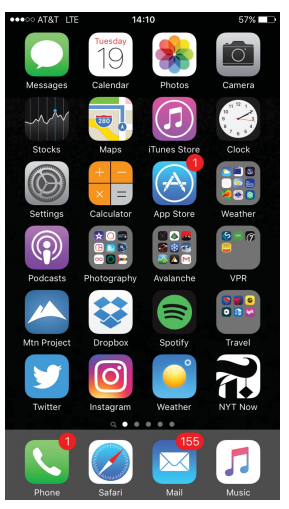
\includegraphics[width = 0.45\textwidth]{images/8.PNG}
\end{center}
Mostriamo ora come passare da un'espressione regolare R ad un $\varepsilon$-NFA E. In particolare, quindi, mostriamo che ogni linguaggio $L$ che sia uguale a $L(R)$ per un'espressione regolare $R$ è anche uguale a $L(E)$ per un $\varepsilon$-NFA E. La dimostrazione avviene per \textbf{induzione strutturale sulla struttura di R}:

\begin{Teorema}
Ogni linguaggio definito da un'espressione regolare è definito anche da un automa a stati finiti
\end{Teorema}

\begin{Dimostrazione}
    Supponiamo che $L = L(R)$ per un'espressione regolare $R$. Mostriamo anche che $L = L(E)$ per un $\varepsilon$-NFA E per induzione con dei "moduli" costruiti nel seguente modo:
    \begin{enumerate}
        \item Uno stato accetante
        \item Nessun arco entrante nello stato iniziale
        \item Nessun arco uscente dallo stato finale
    \end{enumerate}
    Procediamo per induzione sulla struttura di $R$ utilizzando la definizione ricorsiva delle espressioni regolari: (gli archi entranti nel "primo" stato dei moduli \textbf{NON} indicano stati iniziali, ma transizioni da stati "precedenti", potenzialmente dallo stato iniziale dell'automa complessivo) \newline \newline
    \textbf{Casi base}:
    \begin{enumerate}
        \item Se $R = \varepsilon$ $($quindi $L(R) = \{\varepsilon\})$, allora il modulo è il seguente:
            \begin{center}
                \hspace*{-1cm}
                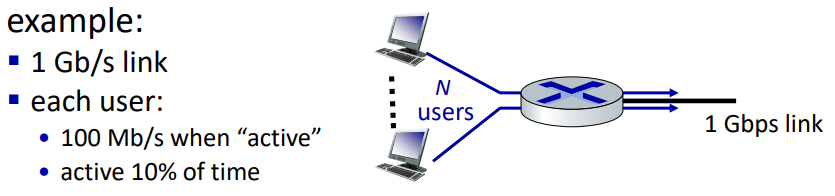
\includegraphics[width = 0.45\textwidth]{images/9.PNG}
            \end{center}
        \item Se $R = \emptyset$ $($quindi $L(\emptyset) = \emptyset)$, allora il modulo è il seguente:
            \begin{center}
                \hspace*{-1cm}
                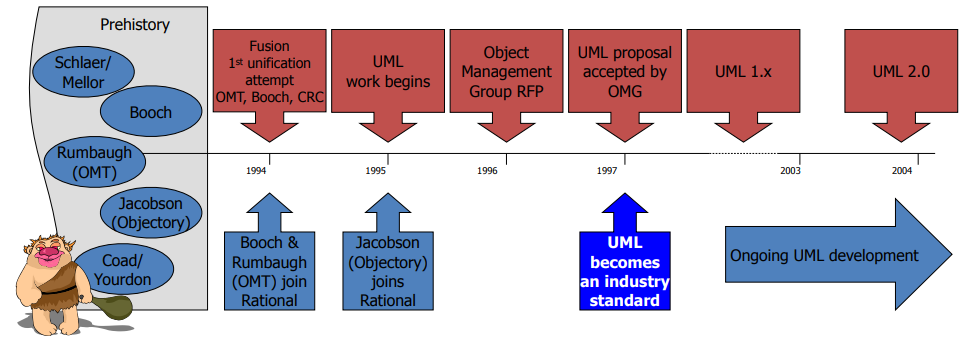
\includegraphics[width = 0.45\textwidth]{images/10.PNG}
            \end{center}
        \item se $R = a$ $($e quindi $L(R) = \{a\})$, allora il modulo è il seguente:
            \begin{center}
                \hspace*{-1cm}
                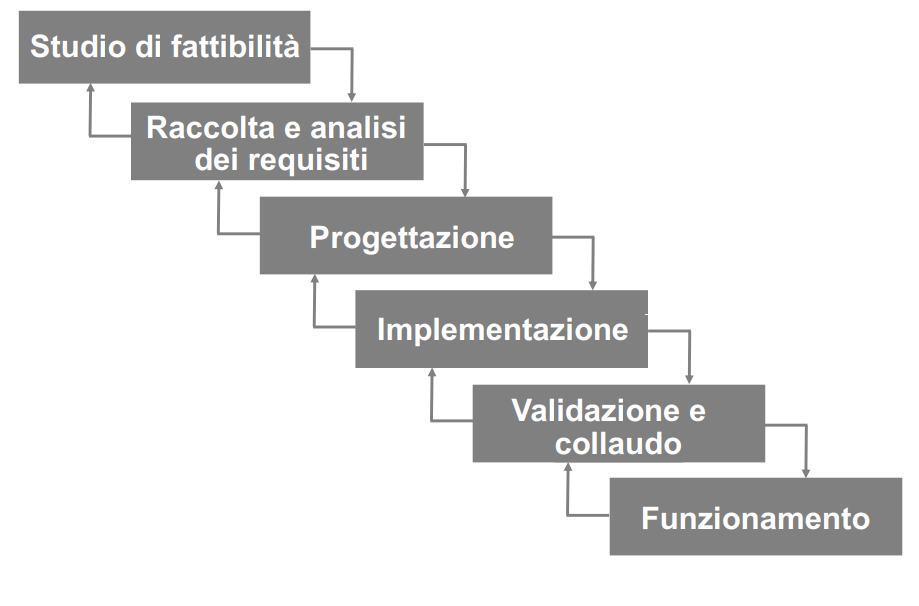
\includegraphics[width = 0.45\textwidth]{images/11.PNG}
            \end{center}
    \end{enumerate}
    \textbf{Passo induttivo}:
    \begin{enumerate}
        \item Se $R = S + T$ $($e quindi $L(R) = L(S) \cup L(T))$ allora il modulo è il seguente:
        \begin{center}
                \hspace*{-1cm}
                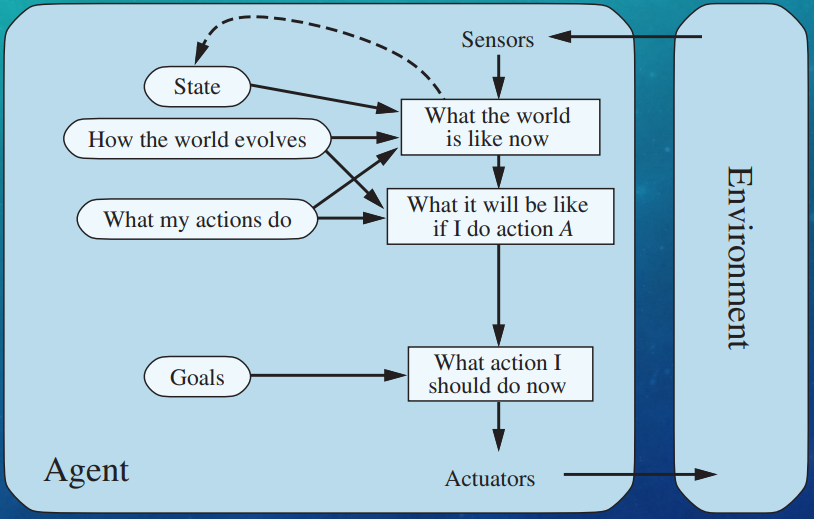
\includegraphics[width = 0.55\textwidth]{images/12.PNG}
        \end{center}
        L'espressione è $S + T$ per due espressioni più piccole $S$ e $T$. Partendo dal nuovo stato iniziale, possiamo andare nello stato iniziale dell'automa per T o nello stato iniziale dell'automa per S. Possiamo quindi arrivare nello stato accetante di uno dei due atomi seguendo un cammino etichettato da una stringa che si trova o in $L(S)$ o in $L(T)$. Una volta arrivati in uno dei due stati accettanti per $L(S)$ o $L(T)$, possiamo usare uno dei due archi $\varepsilon$ per arrivare nello stato accetante del nuovo automa. Il linguaggio riconosciuto è pertanto $L(S) \cup L(T)$

        \item Se $R = ST$ $($e quindi $L(R) = L(S) \circ L(T))$, allora il modulo è il seguente:
        \begin{center}
                \hspace*{-1cm}
                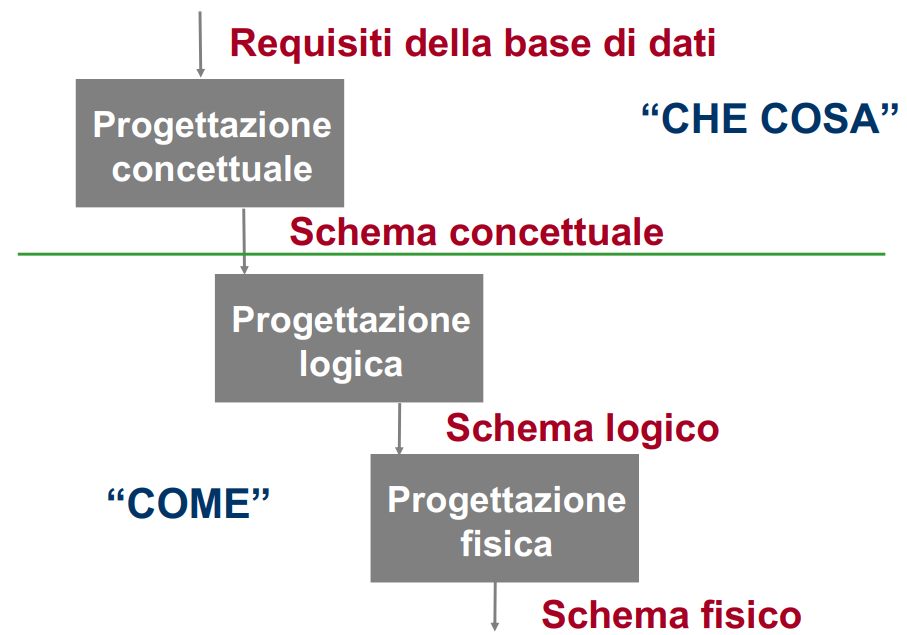
\includegraphics[width = 0.55\textwidth]{images/13.PNG}
        \end{center}
        L'espressione è $ST$ per due espressioni più piccole $S$ e $T$. Si noti come lo stato accettante del 2° automa diventa lo stato accentate per l'automa complessivo. L'idea è che un cammino dallo stato iniziale a quello accettante deve prima seguire un cammino etichettato da una stringa in $L(S)$ e poi un cammino etichettato da una stringa in $L(T)$; quindi i cammini dell'automa sono \textbf{tutti e soli} i cammini etichettati dalle stringhe in $L(S) \circ L(T)$

        \item $R = S^*$ $($quindi $L(R) = (L(S))^*$, allora il modulo è il seguente:
        \begin{center}
                \hspace*{-1cm}
                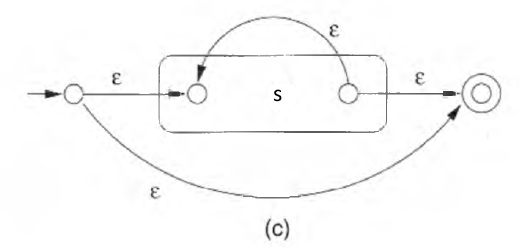
\includegraphics[width = 0.55\textwidth]{images/14.PNG}
        \end{center}
        L'espressione è $S^*$ per un'espressione più piccola $S$. Abbiamo quindi due tipi di percorso:
        \begin{itemize}
            \item Direttamente dal 1° stato del modulo allo stato accettante attraverso una $\varepsilon$-transizione. Tale cammino fa accettare $\varepsilon$, che si trova in $L(S^*)$. a prescindere da $S$.
            \item Si passa per lo stato iniziale dell'automa per $S$, attraverso l'automa una o più volte, e poi verso lo stato accetante. Così facendo, copriamo tutte le stringhe di $L(S^*)$ eccetto $\varepsilon$
        \end{itemize}
        \item $R = (S)$ $($quindi $L(R) = L(S))$, allora il modulo per $R$ è uguale al modulo per $S$.
    \end{enumerate}
    Si osservi quindi che i "moduli" (automi) definiti rispettano le 3 condizioni date nell'ipotesi induttiva.
\end{Dimostrazione}
\subsection{Da DFA a Espressione Regolare tramite eliminazione di stati}
Mostriamo ora la costruzione di un espressione regolare a partire dal DFA che la accetta mediante l'eliminazione di stati. Quando eliminiamo uno stato $s$, tutti i cammini che passano per $s$ non esisteranno più nel nuovo automa; per non cambiare il linguaggio da esso accettato dobbiamo includere, su un arco che va direttamente da uno stato $q$ a uno stato $p$, le etichette dei cammini che vanno da $q$ a $p$ attraverso $s$. Per farlo, etichettiamo gli archi con le \textbf{stringhe} che rappresentano la transizioni. Poiché le transizioni potrebbero essere rappresentate da infinite stringhe, utilizziamo le \textbf{espressioni regolari} per rappresentarle. Siamo dunque portati a considerare automi che hanno come etichette degli archi delle espressioni regolari e il \textbf{linguaggio dell'automa} è l'unione, su tutti i cammini dallo stato iniziale a uno stato accettante, dei linguaggi formati concatenando i linguaggi delle espressioni regolari lungo un cammino. Si noti che questa regola è coerente con la definizione di linguaggio associato ad un qualunque tipo di automa trattato fin qui. Ogni simbolo $a$ o $\varepsilon$ può essere pensato come un'espressione regolare il cui linguaggio è la stringa $\{a\}$ o $\{\varepsilon\}$. Passiamo ora alla descrizione della procedura: consideriamo il seguente automa con uno stato $s$ che vogliamo eliminare:
\begin{center}
    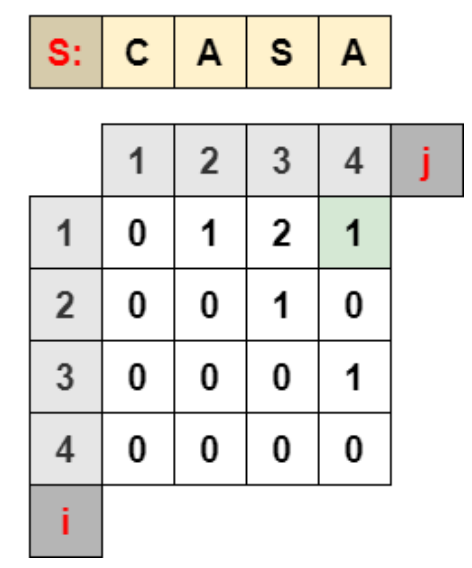
\includegraphics[width = 0.40\textwidth]{images/15.PNG}
\end{center}
Supponiamo che gli stati $q_1, ..., q_k$ siano predecessori di $s$ e gli stati $p_1, ..., p_m$ siano successori di $s$. È possibile che alcuni dei $q$ siano anche fra i $p$, ma supponiamo che $s$ non si trovi tra i $q$ o i $p$, anche se esiste un ciclo da $s$ a se stesso. Mostriamo anche un'espressione regolare su ciascun arco da uno dei $q$ ad $s$; l'espressione $Q_i$ etichetta l'arco uscente da $q_i$. In modo analogo, mostriamo l'espressione regolare $P_i$ che etichetta l'arco da $s$ a $p_i$ per ogni $i$. Mostriamo un ciclo su $s$ con etichetta $S$. Infine, esiste un espressione regolare $R_{ij}$ sull'arco che va da $q_i$ a $p_j$ per tutti i valori di $i$ e $j$. Si osservi che alcuni di questi archi \textbf{potrebbero non esistere nell'automa}, quindi li possiamo pensare come archi etichettati con $\emptyset$. Eliminiamo ora lo stato, portando l'automa in questa forma:
\begin{center}
    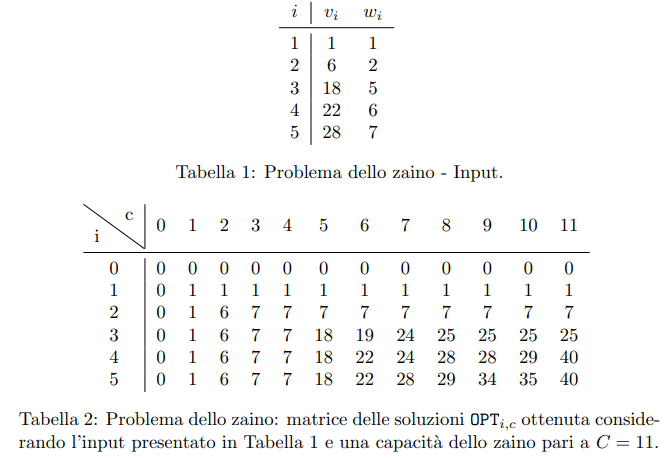
\includegraphics[width = 0.45\textwidth]{images/16.PNG}
\end{center}
Per compensare la cancellazione di $s$, introduciamo per ogni predecessore $q_i$ e ogni successore $p_j$ di $s$ un'espressione regolare che rappresenta tutti i cammini che partono da $q_i$, vanno a $s$, ciclano per 0 o più volte su $s$ e infine vanno a $p_j$. L'espressione per questi cammini è:
$$Q_iS^*P_j$$
Tale espressione viene aggiunta, attraverso l'operatore di unione$(+)$, all'arco da $q_i$ a $p_j$. Se non esiste un arco tra $q_i$ e $p_j$, ne introduciamo prima uno, etichettandolo con l'espressione regolare $\emptyset$. \newline
Descriviamo quindi la procedura per ottenere un'espressione regolare partendo da un'automa a stati finiti:
\begin{enumerate}
    \item Per ogni stato accettante $q$ applichiamo il processo di riduzione visto sopra per produrre un'automa equivalente con le etichette sugli archi costituite da \textbf{espressioni regolari}. \textbf{Eliminiamo tutti gli stati eccetto $q$ e lo stato iniziale $q_0$}.
    \item Se $q \neq q_0$, allora il risultato è un automa a due stati simile al seguente:
        \begin{center}
            \hspace{-2cm}
            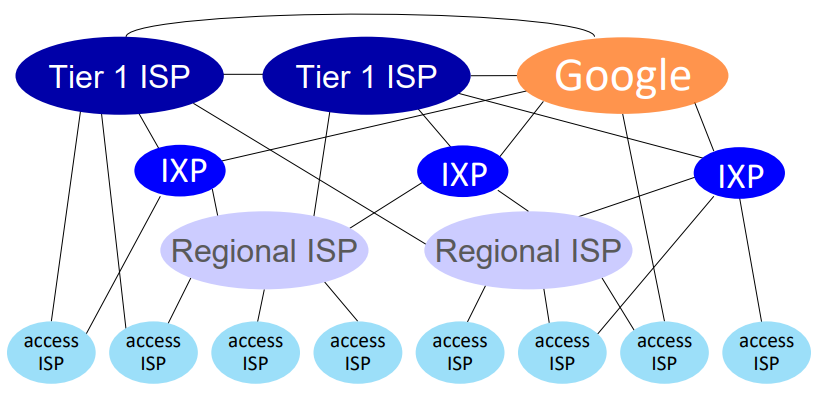
\includegraphics[width = 0.45\textwidth]{images/17.PNG}
        \end{center}
    L'espressione regolare per le stringhe accettate si può descrivere in vari modi, uno dei quali è:
    $$E_i = (R + SU^*T)^* SU^*$$
    \item Se lo stato iniziale è anche accettante, dobbiamo eliminare \textbf{tutti gli stati dell'automa originale}, eccetto quello iniziale. Così facendo otteniamo un automa a uno stato, simile al seguente:
        \begin{center}
            \hspace{-2cm}
            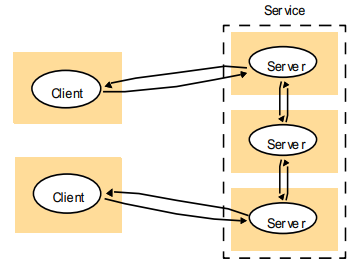
\includegraphics[width = 0.25\textwidth]{images/18.PNG}
        \end{center}
    L'espressione regolare che indica le stringhe accettate dall'automa è la seguente:
    $$E_i = R^*$$
    \item L'espressione regolare desiderata è la somma (unione) di tutte le espressioni regolari derivate dagli automi ridotti \textbf{per ogni stato accettante}, in virtù delle regole (2) e (3).
\end{enumerate}
\subsubsection{Ordine di eliminazione degli stati}
Uno stato viene eliminato in tutti gli automi derivati quando non è né iniziale, né accettante. Perciò, un vantaggio del processo di eliminazione degli stati è che possiamo iniziare eliminando ogni stato che non è né iniziale né accettante. Lo sforzo si duplica se dobbiamo eliminare degli stati accettanti; tuttavia possiamo procedere in questa maniera: supponiamo di avere 3 stati accettanti $p, q, r$. È possibile eliminare $p$, e poi eliminare separatamente $q$ ed $r$, producendo gli automi ridotti rispettivamente per $r$ e $q$. Poi ricominciamo con tutti e 3 gli stati accettanti ed eliminiamo sia $q$ ed $r$, ottenendo l'automa per $p$

\section{Proprietà dei linguaggi regolari}
\subsection{Chiusura dei linguaggi regolari}
Indichiamo con $REG$ la \textbf{classe dei linguaggi regolari} e dimostriamo la loro \textbf{chiusura} rispetto a varie operazioni.
\subsubsection{Chiusura rispetto all'unione, concatenazione e chiusura di Kleene}
\begin{Teorema}
Se $L, M \in REG$, allora $L \cup M \in REG$    
\end{Teorema}

\begin{Dimostrazione}
    Se $L, M$ sono regolari allora esistono due espressioni regolari $R, S$ t.c.
    $L(R) = L, L(S) = M$. Allora $L\cup M = L(R+S)$
\end{Dimostrazione}

\begin{Dimostrazione}[Alternativa]
    Se $L, M \in REG$, allora esistono due automi a stati finiti $R$ ed $S$ che riconoscono rispettivamente $L$ ed $M$. Il seguente $\varepsilon$-NFA riconosce $L\cup M$, quindi esso è regolare.
    \begin{center}
        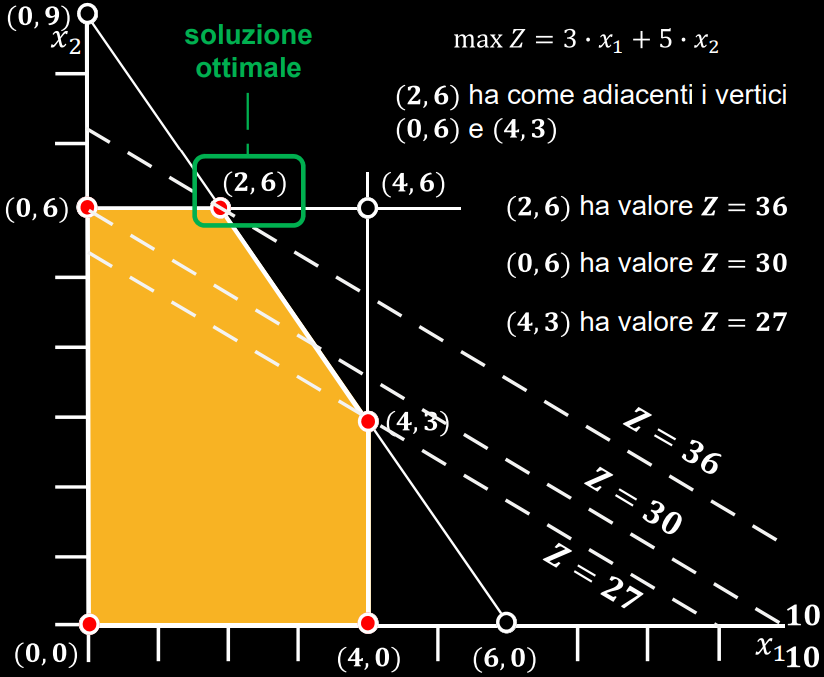
\includegraphics[width = 0.55\textwidth]{images/19.PNG}
    \end{center}
\end{Dimostrazione}
Inoltre, se $L \subseteq \Sigma^*_1$ e $M \subseteq \Sigma^*_2$ il teorema vale ancora? Si poiché $\Sigma = \Sigma_1 \cup \Sigma_2$ quindi $L, M \subseteq \Sigma$

\begin{Teorema}
    Se $L, M \in REG$, allora $LM \in REG$
\end{Teorema}
\begin{Teorema}
    Se $L \in REG, allora \; L^* \in REG$
\end{Teorema}
\subsubsection{Chiusura rispetto alla complementazione}
\begin{Teorema}
    Se $L \in REG$, su $\Sigma \; (L \subseteq \Sigma^*)$, allora anche il complemento di $L$, $\overline{L} = \Sigma^* \backslash L$ è regolare.
\end{Teorema}
\begin{Dimostrazione}
    Se $L\in REG$, allora $\exists DFA \; A = (Q, \Sigma, \delta, q_0, F)$ t.c. $L$ è il linguaggio accettato da $A$. Allora $\overline{L} = L(B)$ dove $B$ è il DFA:
    $$B = (Q, \Sigma, \delta, q_0, Q \backslash F)$$
\end{Dimostrazione}
\begin{Osservazione}
    $\overline{L}$ dipende dall'alfabeto $\Sigma$. Quindi $\overline{L} = \Sigma^* \backslash L$. Se definisco $L$ su $\Sigma \subset \Gamma$, allora il complemento sarà $\overline{L} = \Gamma^* \backslash L$
\end{Osservazione}
\begin{Proposizione}
    La cardinalità di $\Sigma$ e $\Gamma$ è isomorfa alla cardinalità dei numeri naturali:
    $$|\mathbb{N}| = \aleph_0$$
\end{Proposizione}
Come costruiamo una ER per $\overline{L}$ partendo da una ER per $L$? Possiamo questa procedura:
\begin{enumerate}
    \item Costruiamo l'$\varepsilon$-NFA per $L$
    \item Convertiamo l'$\varepsilon$-NFA per $L$ in DFA
    \item Trasformiamo gli stati finali del DFA in stati non finali e viceversa, ottenendo il DFA per $\overline{L}$
    \item Ricostruiamo l'ER per $\overline{L}$ attraverso la procedura di eliminazione degli stati.
\end{enumerate}
\subsubsection{Chiusura rispetto all'intersezione}
\begin{Teorema}
    Se $L, M \in REG$, allora $L \cap M \in REG$ (su $\Sigma$).
\end{Teorema}
\begin{Dimostrazione}
    Per le leggi di De Morgan:
    $$L \cap M = \overline{\overline{L} \cup \overline{M}}, \overline{L}\in REG, \overline{M}\in REG, \overline{L} \cup \overline{M}\in REG$$
    $$\overline{\overline{L} \cup \overline{M}} \in REG$$
\end{Dimostrazione}
\subsubsection{Chiusura rispetto alla differenza insiemistica}
\begin{Teorema}
    Se $L, M \in REG$, allora $L \backslash M \in REG$
\end{Teorema}
\begin{Dimostrazione}
    Vale $L \backslash M = L \cap \overline{M}$. Poiché $M \in REG$ allora $\overline{M} \in REG$, quindi anche $L \cap \overline{M} \in REG$
\end{Dimostrazione}
\subsection{Equivalenza e minimizzazione di automi}
Prima di presentare il processo di minimizzazione di un DFA, diamo prima qualche nozione preliminare:
\subsubsection{Relazioni di equivalenza tra stati}
\begin{Definizione}
    Dati due stati $p$ e $q$, essi sono \textbf{equivalenti} se per ogni stringa $w \in \Sigma^*$, $\hat{\delta}(p, w) \in F \Leftrightarrow \hat{\delta}(q, w) \in F$(quindi entrambi finali o non finali)
\end{Definizione}
Se $p$ e $q$ sono equivalenti, allora lo indicheremo con $p \approx q$. In caso non lo siano, lo indicheremo con $p \not\approx q$.
\begin{Teorema}
    $\approx$ è una relazione di equivalenza su Q.
\end{Teorema}
\begin{Dimostrazione}
    La relazione è:
    \begin{itemize}
        \item \textbf{Riflessiva}: $p \approx p \; \forall p \in Q$
        \item \textbf{Simmetrica}: Se $p \approx q$ allora $q \approx p \; \forall p,q \in Q$
        \item \textbf{Transitiva}: Se $p \approx q$ e $q \approx r$ allora $p \approx r \; \forall p,q,r\in Q$
    \end{itemize}
\end{Dimostrazione}
Quindi $\approx$ determina delle \textbf{classi di equivalenza} su $Q$. Le classi di equivalenza sono tra loro \textbf{disgiunte}, cioè non vi è nessun elemento che può appartenere a due classi di equivalenza distinte. \newline
Tutti gli elementi appartengono ad una classe di equivalenza; l'insieme di tutte le classi di equivalenza forma una \textbf{partizione di Q}.
\begin{Nota}
    Se vogliamo dimostrare che $p \not\approx q$, basta trovare una stringa $w \in \Sigma^*$ t.c. $\hat{\delta}(p, w) \in F$ ma $\hat{\delta}(q, w) \not\in F$. Se esiste, tale stringa è detta \textbf{testimone} del fatto che $p \not\approx q$. Se due stati non sono equivalenti si dicono \textbf{distinguibili}
\end{Nota}
Per trovare gli stati equivalenti dobbiamo prima conoscere gli stati \textbf{distinguibili}; per trovarli applichiamo \textbf{l'algoritmo riempi-tabella}:
\begin{Proposizione} \hphantom{0}
    \begin{itemize}
        \item \textbf{Base}: Se $p$ è uno stato accettante e $q$ non è uno stato accettante, allora la coppia $\{p, q\}$ è distinguibile.
        \item \textbf{Induzione}: Siano $p$ e $q$ due stati tali che, per un simbolo di input $a$, $r = \delta(p, a)$ e $s = \delta(q, a)$ sono stati che sappiamo essere distinguibili. Allora $\{p, q\}$ sono distinguibili. La regola vale perché dev'esserci una stringa $w$ che distingue $r$ ed $s$; in altre parole solo uno tra $\hat{\delta}(r, w)$ e $\hat{\delta}(s, w)$ è accettante. Ma allora la stringa $ax$ distingue $p$ da $q$ perché $\hat{\delta}(p, aw)$ e $\hat{\delta}(q, aw)$ coincidono rispettivamente con $\hat{\delta}(r, w)$ e $\hat{\delta}(s, w)$
    \end{itemize}
\end{Proposizione}
O in altre parole:
\begin{enumerate}
    \item Creo una tabella con tutte le combinazioni tra gli stati dell'automa; evitando i controlli duplicati
    \item Metto un segno nella tabella per ogni coppia di stati "immediatamente" distinguibile; cioè per ogni coppia per la quale il testimone ha lunghezza 1.
    \item Aumento la lunghezza del testimone cercato e itero il punto 2; se metto almeno un segno, itero di nuovo l'algoritmo; altrimenti termino
\end{enumerate}
\begin{center}
    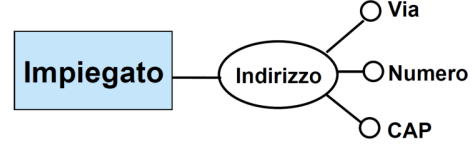
\includegraphics[width = 0.35\textwidth]{images/20.PNG}
\end{center}
\begin{Teorema}
    Se due stati non sono distinti dall'algoritmo riempi-tabella, allora \textbf{sono equivalenti}
\end{Teorema}
Possiamo ora costruire l'automa minimo, i quali stati sono le \textbf{classi di equivalenza}
\begin{Osservazione}
    Non ci può essere una classe di equivalenza che contiene stati finali e non finali
\end{Osservazione}
\begin{Proposizione}
    Per costruire l'automa minimo e applicare l'algoritmo riempi-tabella, è necessario eliminare gli \textbf{stati non raggiungibili} prima di procedere.
\end{Proposizione}
\begin{Proposizione}
    La relazione di equivaelnza $\approx$ è \textbf{stabile} rispetto alla $\delta$, cioè prendendo un rappresentate di classe qualsiasi e calcolandone la $\delta$ si finisce sempre in un elemento appartenente ad una classe di equivalenza
\end{Proposizione}
\begin{Proposizione}
    L'automa minimo è \textbf{unico}
\end{Proposizione}
\subsection{Equivalenza di linguaggi regolari}
Siano $L, M \in REG$. Essendo regolari, esistono due DFA $A_L$ e $A_M$:
$$A_L = (Q_L, \Sigma, \delta_L, q_L, F_L)$$
$$A_M = (Q_M, \Sigma, \delta_M, q_M, F_M)$$
Costruiamo un nuovo automa $A$:
$$A = (Q_L \cup Q_M, \Sigma, \delta, q_L, F_L \cup F_M)$$
Con $\delta$ che si comporta come $\delta_L$ sul "diagramma degli stati" di $A_L$ e come $\delta_M$ sul "diagramma degli stati" di $A_M$. Quindi:
$$L = M \Leftrightarrow q_L \approx q_M \;$$ cioe' 
$$\Leftrightarrow \forall w \in \Sigma^*, \hat{\delta}(q_L, w) \in F_L \Leftrightarrow \hat{\delta}(q_M, w)\in F_M \;$$ cioe' \newline
$\Leftrightarrow w$ è accettata sia da $A_L$ che da $A_M$ oppure è rifiutata da entrambi. Per scoprire se i due automi sono uguali posso quindi applicare l'algoritmo riempi-tabella su $A$.
\begin{Nota}
    Se, con una stringa $w$, il segno finisce in una coppia con già un segno per lo stesso simbolo, allora sono \textbf{distinguibili}
\end{Nota}
\subsection{Tempi di calcolo dell'algoritmo riempi-tabella}
Sia $Q$ l'insieme di stati di un DFA. Allora $|Q| = n$ e $|Q \times Q| = n^2$. Durante l'esecuzione dell'algoritmo riempi-tabella analizziamo un numero di coppie distinte $(p, q)$ uguale a $n^2$. Ciò vuol dire che: \newline
\textbf{Complessità temporale ad ogni passo intermedio}: $O(n^2)$ \newline
\textbf{Complessità temporale totale}: $O(n^4)$
\begin{Nota}
    In verità, con una struttura dati che permetta l'accesso diretto alle celle vuote della tabella, si hanno tempi di calcolo leggermente ridotti; ma sempre nell'ordine di quanto riportato sopra.
\end{Nota}
\subsection{Perché il DFA minimo non può essere migliorato}
Supponiamo di minimizzare un DFA $A$ con l'algoritmo riempi-tabella e di ottenere come risultato un DFA $M$. Può esistere un $DFA$ N che accetta lo stesso linguaggio di $A$ e di $M$ ma con un numero di stati minore di $M$? La risposta è no:
\begin{Dimostrazione}
    Cominciamo eseguendo la procedura per riconoscere gli stati \textbf{distinguibili} sugli stati di $M$ ed $N$, come se fossero un solo DFA. Possiamo suppore che i nomi degli stati di $M$ siano distinti da quelli di $N$; in questo modo, la funzione di transizione $\delta$ dell'automa composto è \textbf{l'unione delle due funzioni}, senza interferenze. Un stato è accettante nel DFA composto se e solo se è accettante nel DFA di provenienza.
    Gli stati iniziali di $M$ ed $N$ sono \textbf{indistinguibili} poiché $L(M) = L(N)$; inoltre, se $p$ e $q$ sono indistinguibili, lo sono anche i loro successori per qualsiasi simbolo di input: infatti, se potessimo distinguere i loro successori, potremmo anche distinguere $p$ e $q$. Né $M$ né $N$ hanno stati \textbf{inaccessibili}; in caso contrario, possiamo eliminarli ed ottenere un DFA più piccolo per lo stesso linguaggio. \newline
    Perciò, ogni stato di $M$ è \textbf{indistinguibile} da almeno uno stato di $N$. Per convincersene, sia $p$ uno stato di $M$. Deve esistere una stringa $a_1a_2...a_k$ che porta dallo stato iniziale di $M$ a $p$. La stessa stringa porta anche dallo stato iniziale di $N$ a uno stato $q$. Sappiamo che gli stati iniziali sono \textbf{indistinguibili}, quindi anche i loro successori rispetto ad $a_1$ sono \textbf{indistinguibili}; lo stesso vale per i successori di questi stati rispetto ad $a_2$ e così via, fino a concludere che $p$ e $q$ sono indistinguibili.
    Poiché $N$ ha \textbf{meno stati} di $M$, ci sono due stati di $M$ \textbf{indistinguibili} dallo stesso stato di $N$, e quindi \textbf{indistinguibili fra loro}. Ma $M$ è stato costruito come essere l'automa minimo, quindi esso deve avere tutti i suoi stati \textbf{distinguibili fra loro a due a due}; abbiamo quindi un assurdo! Quindi \textbf{non può esistere $N$} ed $M$ ha un numero di stati \textbf{non superiore} a quello di un qualsiasi DFA equivalente ad $A$
\end{Dimostrazione}
In termini formali, abbiamo dimostrato il seguente teorema:
\begin{Teorema}
    Sia $A$ un DFA ed $M$ il DFA costruito a partire da $A$ applicando l'algoritmo riempi-tabella. Allora il numero di stati di $M$ non è superiore a quello di un qualsiasi DFA equivalente ad $A$.
\end{Teorema}
Possiamo inoltre affermare che, con la dimostrazione precedente, abbiamo provato che esiste una corrispondenza \textbf{uno-a-uno} fra gli stati di due automi minimi $N$ ed $M$. Poiché abbiamo dimostrato che ogni stato di $M$ deve essere equivalente ad un solo stato di $N$ e che non può essere equivalente a due o più stati di $N$; allora possiamo facilmente dimostrare, in maniera simile, il contrario. In conclusione, quindi, vale il seguente teorema:
\begin{Teorema}
    Il DFA minimo equivalente ad $A$ è \textbf{unico}, a meno di rinominare gli stati
\end{Teorema}
\subsubsection{Perché l'algoritmo riempi-tabella non funziona sugli NFA}
Si potrebbe pensare che l'algoritmo riempi-tabella possa essere applicato anche per la ricerca di NFA minimi a DFA assegnati. Invece, anche se è possibile trovare un NFA con numero minimo di stati che accetta un determinato linguaggio, non è sufficiente ripartire gli stati di un NFA per quel linguaggio. Facciamo un esempio:
\begin{center}
    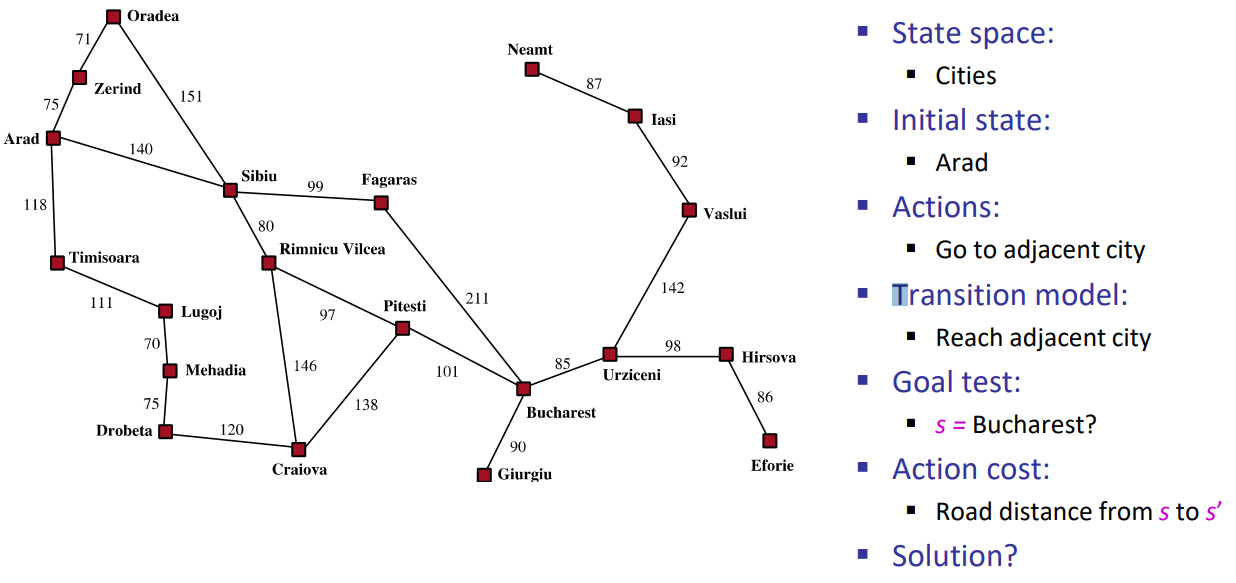
\includegraphics[width = 0.35\textwidth]{images/21.PNG}
\end{center}
In questo NFA, \textbf{non ci sono coppie di stati equivalenti}; $B$ è di sicuro distinguibile da $A$ e $C$; $A$ e $C$ sono distinguibili per l'input $0$; $A$ è l'unico successore di $C$ e non è accettante, mentre l'insieme dei successori di $A$ è $\{A, B\}$, che contiene uno stato accettante. Perciò, non si può ridurre il numero di stati raggruppando quelli equivalenti. Eppure, si può trovare un NFA più piccolo per questo linguaggio \textbf{rimuovendo $C$}; infatti, i soli stati $A$ e $B$ accettano tutte le stringhe del linguaggio e l'aggiunta di $C$ non permette di accettare altre stringhe.
\subsection{Pumping Lemma}
Il Pumping Lemma è un teorema(Lemma) che permette di \textbf{dimostrare}, procedendo per assurdo, che un certo linguaggio $L$ non è regolare.
\begin{Nota}
    Le \textbf{prefisse} di una stringa sono le stringhe ottenute rimuovendo simboli dalla fine della stringa.
\end{Nota}
Consideriamo il linugaggio:
$$L_{01} = \{0^n 1^n |n \geq 1 \}$$
Vogliamo dimostrare che è regolare. Se per assurdo, $L_{01}$ fosse regolare, allora esisterebbe un DFA che lo accetta. Sia quindi $A = (Q, \Sigma, \delta, q_0, F)$ e supponiamo che $|Q| = k$. Diamo in input ad $A$ la stringa $0^{k}$; essa ha $k + 1$ prefisse $(\varepsilon, 0, 00, 000...)$ Poiché ci sono $k$ stati, devono esistere due prefisse \textbf{diverse}, $0^i$ e $0^j$, con $i \neq j$, che portano allo stesso stato, \textbf{quindi non sono distinguibili}. $A$ deve accettare $0^i1^i$ poiché appartiene al linguaggio, tuttavia accetterebbe anche $0^j1^i$, e quindi \textbf{sbaglia}; quindi $A$ non può esistere e $L_{01}$ non è regolare.
\begin{Teorema}
    Sia $L$ un linguaggio regolare, allora esiste una costante $n$ (dipendente da $L$) t.c. $\forall w \in L$ t.c. $|w| \geq n$, allora $w$ può essere scomposta come $w = xyz$ in modo che valgano:
    \begin{enumerate}
        \item $y \neq \varepsilon$
        \item $|xy| \leq n$
        \item $\forall k \geq 0$, anche $xy^kz \in L$
    \end{enumerate}
\end{Teorema}
\begin{Dimostrazione}
    Se $L \in REG$, allora esiste un DFA $A$ che lo riconosce. Supponiamo che $A$ abbia $n$ stati e consideriamo una stringa $w = a_1a_2...a_m$ t.c. $m \geq n$ (quindi $|w| \geq n$) con $a_i \in \Sigma \; \forall i = 1,...,m$. Per ogni $i = 0,...,n$, sia $p_i = \hat{\delta}(q_0, a_1,...,a_i)$. Avremo che $p_0 = q_0$. Dato che $A$ ha $n$ stati, gli $n+1$ stati $p_0, p_1,...,p_n$ non possono essere tutti distinti. Allora $\exists i,j$ con $0\leq i < j \leq n$ tali che $p_i = p_j$. Scomponiamo $w = xyz$, allora:
    \begin{enumerate}
        \item $x = a_1...a_i$
        \item $y = a_{i+1}...a_j$
        \item $z = a_{j+1}...a_m$
    \end{enumerate}
\end{Dimostrazione}
In altre parole, $x$ porta fino a $p_i$, y porta fino a $p_j$, il quale coincide con $p_i$ e infine $z$ conclude $w$. Le relazioni fra stati e stringhe sono rappresentabili con il seguente automa: (il cappio indica una qualsiasi cammino che ritorna a $p_i$):
\begin{center}
    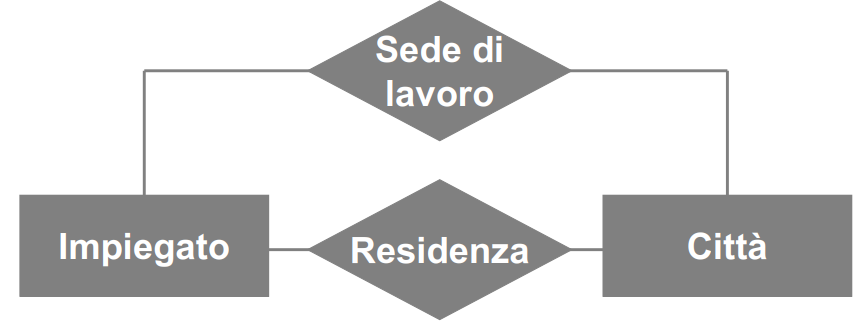
\includegraphics[width = 0.65\textwidth]{images/22.PNG}
\end{center}
Consideriamo ora cosa accade se l'automa riceve in input la stringa $xy^kz$ per $k \geq 0$. Se $k = 0$, l'automa passa dallo stato iniziale allo stato $p_i$ sull'input $x$. Poiché $p_i$ coincide con $p_j$, l'automa deve passare allo stato accettante sull'input $z$, quindi l'automa accetta $xz$. \newline
Se $k > 0$, $A$ va da $p_0$ in $p_i$ su input $x$, cicla su $p_i$ per $k$ volte e poi passa allo stato finale su input $z$, quindi l'automa accetta la stringa $xy^kz$. La stringa $w$ quindi soddisfa le proprietà enunciate nel teorema.

\section{Automi a Pila}
Un automa a Pila o PDA è essenzialmente un automa \textbf{non deterministico} dotato di uno \textbf{stack} nel quale memorizzare una stringa di simboli. A differenza degli automi a stati finiti, grazie allo stack l'automa può ricordare una sequenza potenzialmente \textbf{infinita} di caratteri, tuttavia esso può accedervi solo in ordine \textbf{LIFO}. In generale, gli automi a pila riconoscono \textbf{tutti e soli i linguaggi liberi dal contesto} (Context-Free) 
\begin{center}
    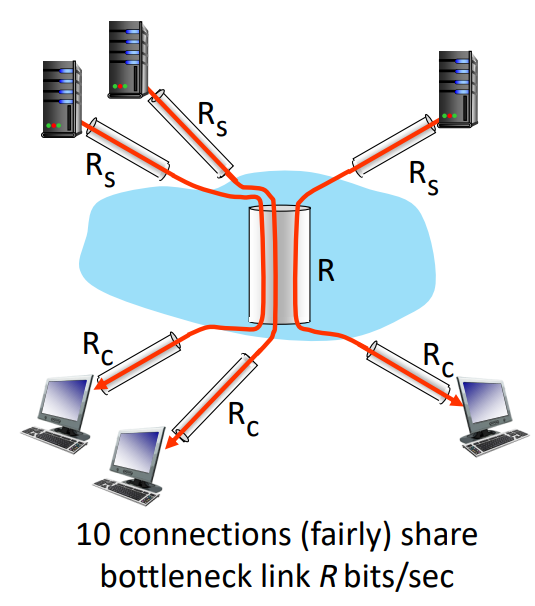
\includegraphics[width = 0.55\textwidth]{images/23.PNG}
\end{center}
Dotiamo questo stack di 3 operazioni fondamentali:
\begin{enumerate}
    \item \textbf{Push}: Immette un simbolo nella pila
    \item \textbf{Pop}: Estrae un simbolo dalla pila
    \item \textbf{Top}: Controlla cosa c'è in cima alla pila
\end{enumerate}
\newpage
\begin{Definizione}
    Un PDA è una 7-upla:
    $$P = (Q, \Sigma, \Gamma, \delta, q_0, z_0, F)$$
    Dove:
    \begin{itemize}
        \item $Q$ è l'insieme finito degli stati
        \item $\Sigma$ è l'insieme dei simboli in ingresso
        \item $\Gamma$ è l'insieme dei simboli della pila
        \item $\delta$ è la funzione di transizione degli stati
        \item $q_0 \in Q$ è lo stato iniziale
        \item $z_0 \in \Gamma \backslash \Sigma$ è un simbolo che indica che la pila è \textbf{logicamente vuota}. Esso viene introdotto poiché la funzione $\delta$ ha bisogno che ci sia \textbf{almeno un simbolo in cima alla pila} per effettuare le sue operazioni. Se vogliamo terminare la computazione, \textbf{rimuoviamo} $z_0$ dalla pila.
        \item F è l'insieme degli stati finali
    \end{itemize}
\end{Definizione}
Definiamo ora la funzione di transizione $\delta$:
$$\delta: Q \times (\Sigma \cup \{\varepsilon\}) \times \Gamma \rightarrow 2^{Q \times \Gamma^*}$$
Dove:
\begin{itemize}
    \item $Q$ è lo stato attuale dell'automa
    \item $(\Sigma \cup \{\varepsilon\})$ è il simbolo in ingresso, appartenente a $\Sigma$ oppure $\varepsilon$
    \item $\Gamma$ è il simbolo \textbf{correntemente in cima alla pila}
\end{itemize}
La funzione di transizione restituisce un \textbf{insieme di coppie} $(q, \gamma)$ dove $q$ è il nuovo stato dell'automa e $\gamma$ è la stringa di simboli che vanno a rimpiazzare la cima dello stack (elencati da sinistra verso destra). Per rimuovere un elemento dalla pila, lo si sostituisce con $\varepsilon$.
\begin{Nota}
    Possiamo aggiungere più stringhe alla pila, ma possiamo togliere un carattere alla volta.
\end{Nota}
\subsection{Notazione grafica per i PDA}
Per costruire il diagramma di transizione per un PDA, si seguono le seguenti regole:
\begin{enumerate}
    \item I nodi corrispondono agli stati del PDA
    \item Una freccia etichettata \textbf{START} indica lo stato iniziale, mentre gli stati contrassegnati da un doppio cerchio sono finali
    \item Gli archi corrispondono alle transizioni del PDA. In particolare, le etichette degli archi sono della forma $a, X/\alpha$, dove $a$ è il simbolo in input, $X$ è il simbolo \textbf{correntemente in cima alla pila} e $\alpha$ è la stringa che verrà immessa in cima alla pila effettuando quella transizione.
\end{enumerate}
\begin{center}
    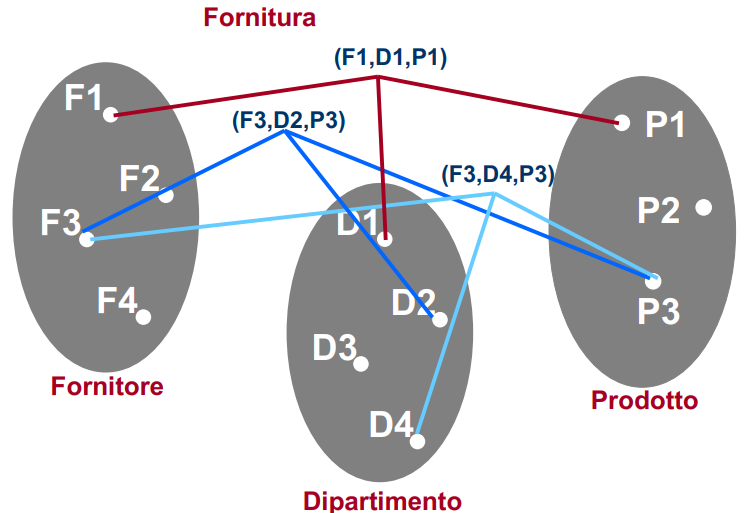
\includegraphics[width = 0.55\textwidth]{images/24.PNG}
\end{center}
\subsection{Configurazioni di un PDA}
\begin{Notazione}
    Configurazione di un PDA $=$ Descrizione istantantea di un PDA (ID)
\end{Notazione}
Finora abbiamo dato solo una vaga nozione di come un PDA computa. Intuitivamente, il PDA passa da una configurazione all'altra reagendo ai vari simboli di input ma, diversamente dagli automi a stati finiti, la configurazione di un PDA comprende anche \textbf{il contenuto dello stack}. Essendo di grandezza arbitraria, lo stack è spesso la parte più importante della configurazione. Rappresentiamo quindi la configurazione di un PDA come una \textbf{tripla} $(q, w, \gamma)$ con $q$ lo stato attuale del PDA, $w$ "l'input residuo" e $\gamma$ il contenuto della pila. Per convenzione, mostriamo la sommità dello stack all'estremo sinistro e il fondo all'estremo destro della stringa $\gamma$.
\subsubsection{Passo di computazione}
Per indicare il passo di computazione (o "mossa") di un PDA e il suo cambio di ID definiamo un nuovo simbolo: $\vdash_P$ (se il PDA ha nome $P$)
\begin{Definizione}
    Dato un PDA $P = (Q, \Sigma, \Gamma, \delta, q_0, z_0, F)$, supponiamo che $\delta(q, a, x)$ contenga $(p, \alpha)$; allora $\forall w \in \Sigma^*$ e $\forall \beta \in \Gamma^*$
    $$(q, aw, x\beta) \vdash_P (p, w, \alpha\beta)$$
\end{Definizione}
\begin{Nota}
    L'insieme di coppie di output di $\delta$ \textbf{deve} essere finito; ciò è importante specificarlo poiché seppur il dominio è \textbf{infinito}, l'insieme $2^{Q \times \Gamma^*}$ è \textbf{potenzialmente infinito}
\end{Nota}
\begin{Nota}
    La definizione di computazione mette in relazione due ID $\Leftrightarrow$ sono legati da un passo di computazione di un caso della $\delta$. Quindi $\vdash$ è una \textbf{relazione binaria} tra due configurazioni legate da un \textbf{passo di computazione}
\end{Nota}
\begin{Definizione}
    Dato un PDA $P = (Q, \Sigma, \Gamma, \delta, q_0, z_0, F)$ e date due sue configurazioni $I$ e $J$, se $I \vdash^*_P J$, si dice allora che $J$ è raggiungibile da $I$ \textbf{in zero o più passi di computazione}(o mosse). La definizione procede per induzione:
    \begin{itemize}
        \item \textbf{Caso base}: $I \vdash^*_P I$ per ogni ID $I$
        \item \textbf{Passo induttivo}: $I \vdash^*_P J$ se $\exists \; ID \; K$ t.c. $I \vdash_P K$ e $K \vdash^*_P J$
    \end{itemize}
    La definizione può essere anche data senza utilizzare l'induzione: \newline
    $I \vdash^*_P J$ se esiste una sequenza di ID $K_1, K_2, ..., K_n$ t.c.:
    \begin{itemize}
        \item $I = K_1$
        \item $J = K_n$
        \item $\forall i = 1,...,n-1,$ $K_i \vdash_P K_{i+1}$
    \end{itemize}
    Quindi $I = K_1 \vdash K_2 \vdash ... \vdash K_{n-1} \vdash K_n = J$
\end{Definizione}
Tramite le ID possiamo quindi costruire anche un \textbf{albero di computazione}, così da mostrare ogni possible computazione e ogni possibile scelta non deterministica che l'automa può fare in ogni suo possibile stato:
\begin{center}
    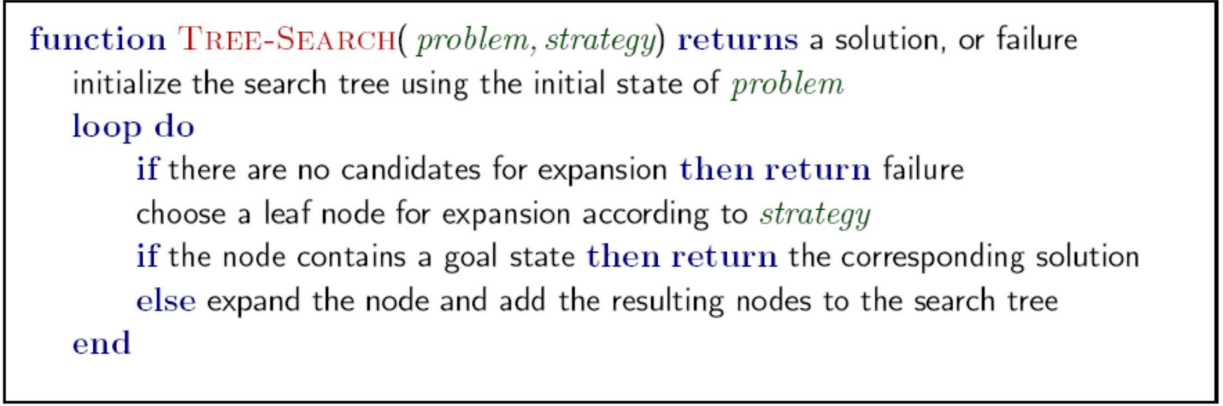
\includegraphics[width = 0.55\textwidth]{images/25.PNG}
\end{center}
\begin{Teorema}
    Se $P = (Q, \Sigma, \Gamma, \delta, q_0, z_0, F)$ è un PDA e $(q, x, \alpha) \vdash^*_P (p, y, \beta)$ allora $\forall w \in \Sigma^*$ e $\forall \gamma \in \Gamma^*$ vale che:
    $$(q, xw, \alpha\gamma) \vdash^*_P (p, yw, \beta\gamma)$$
\end{Teorema}
\begin{Teorema}
    Se $P = (Q, \Sigma, \Gamma, \delta, q_0, z_0, F)$ e $(q, xw, \alpha) \vdash^*_P (p, yw, \beta)$ allora vale anche:
    $$(q, x, \alpha) \vdash^*_P (p, y, \beta)$$
\end{Teorema}
\subsection{Accettazione da parte di un PDA}
\subsubsection{Accettazione per stati finali}
Sia $P = (Q, \Sigma, \Gamma, \delta, q_0, z_0, F)$ un PDA. Il linguaggio accettato da $P$ per \textbf{stato finale} è:
$$L(P) = \{w \in \Sigma^*|(q_0, w, z_0) \vdash^*_P (q, \varepsilon, \alpha) \; con \; q \in F \; e \; \alpha \in \Gamma^*\}$$
\subsubsection{Accettazione per pila vuota}
Sia $P = (Q, \Sigma, \Gamma, \delta, q_0, z_0, F)$ un PDA. Il linguaggio accettato da $P$ per \textbf{pila vuota} è:
$$N(P) = \{w \in \Sigma^*|(q_0, w, z_0) \vdash^*_P (q, \varepsilon, \varepsilon) \; con \; q \in Q\}$$
Se stiamo considerando un PDA che accetta per pila vuota, allora possiamo \textbf{omettere} l'insieme degli stati finali $F$; portando il PDA ad essere una sestupla del tipo:
$$P = (Q, \Sigma, \Gamma, \delta, q_0, z_0)$$
\subsubsection{Da accettazione per pila vuota a per stati finali}
\begin{Teorema}
    Se $L$ è un linguaggio t.c $L = N(P_N)$ per un PDA $P_N = (Q, \Sigma, \Gamma, \delta, q_0, z_0)$ allora esiste un PDA $P_F$ t.c $L = L(P_F)$ 
\end{Teorema}
\begin{Dimostrazione}
    L'idea su cui poggia la dimostrazione è l'utilizzo di un nuovo simbolo $x_0$ che non appartiene a $\Gamma$; $x_0$ è sia il simbolo iniziale di $P_F$ sia il simbolo che indica quando $P_N$ ha svuotato lo stack sullo stesso input. Quindi, $P_F$ avrà la seguente struttura:
    \begin{itemize}
        \item Un nuovo stato iniziale $p_0$ che, tramite una $\varepsilon$-transizione dia il controllo al controllo finito di $P_N$ e che metta sullo stack il simbolo iniziale di $P_N$ $z_0$
        \item Il controllo finito di $P_N$ viene modificato, tracciando un arco ad un nuovo stato finale $p_f$ in ogni stato dove, su un certo input, lo stack verrebbe svuotato.
    \end{itemize}
    In generale, quindi, $P_F$ simula $P_N$ fino a quando lo stack di $P_N$ è vuoto, condizione che porta al nuovo stato accettante $p_f$
\end{Dimostrazione}
\begin{center}
    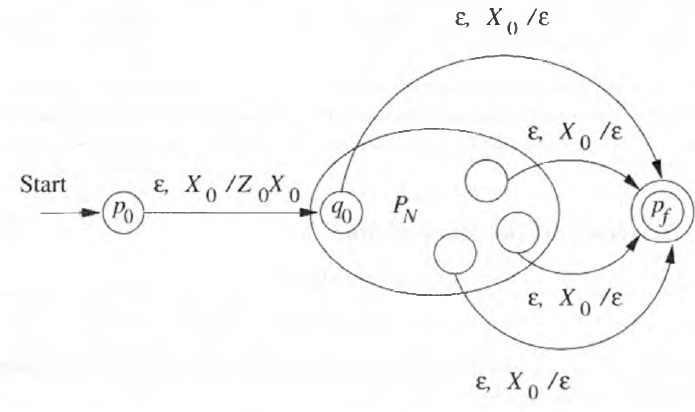
\includegraphics[width = 0.65\textwidth]{images/26.PNG}
\end{center}
La definizione formale del nuovo automa $P_F$ è quindi la seguente:
$$P_F = (Q \cup \{p_0, p_f\}, \Sigma, \Gamma \cup \{x_0\}, \delta_F, p_0, x_0, \{p_F\})$$
Con $\delta_F$ definita nel seguente modo:
\begin{itemize}
    \item $\delta_F(p_0, \varepsilon, x_0) = \{(q_0, z_0,x_0)\}$
    \item $\forall q \in Q, \; \forall a \in \Sigma (o \; a = \varepsilon) \; e \; \forall y \in \Gamma \; \delta_F(q, a, y)$ contiene tutte le coppie di $\delta(q, a, y)$. Inoltre, $\delta_F(q, \varepsilon, x_0)$ contiene $(p_f, \varepsilon)$
\end{itemize}
\subsubsection{Da accettazione per stati finali a per pila vuota}
\begin{Teorema}
    Sia $L = L(P_F)$ per un PDA $P_F = (Q, \Sigma, \Gamma, \delta_F, q_0, z_0, F)$. Allora esiste un automa $P_N$ t.c. $L = N(P_N)$
\end{Teorema}
\begin{Dimostrazione}
    Costruiamo il nuovo automa $P_N$ come suggerito nella seguente figura:
    \begin{center}
        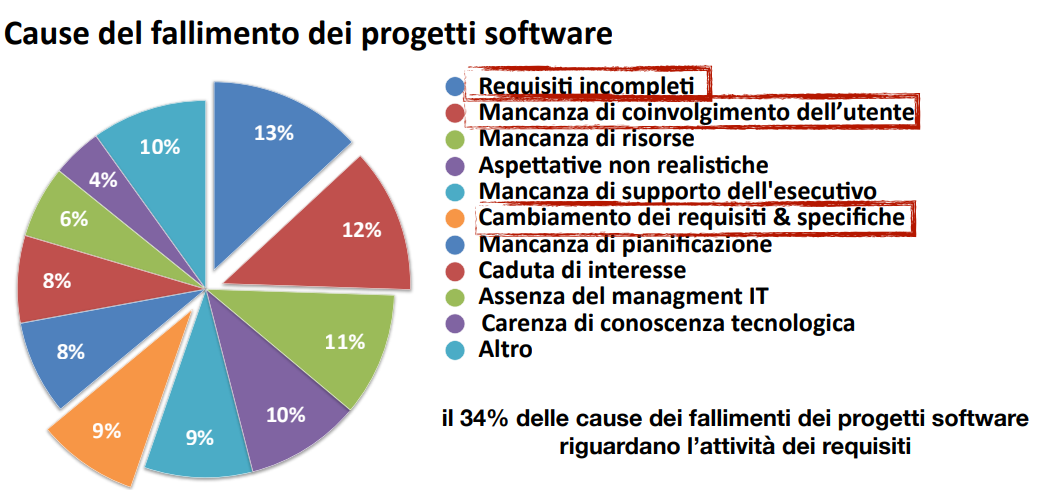
\includegraphics[width = 0.70\textwidth]{images/27.PNG}
    \end{center}
    Quindi sia $P_N = (Q\cup \{p_0, p\}, \Sigma, \Gamma \cup \{x_0\}, \delta_N, p_0, x_0)$ \newline
    Con $\delta_N$ definita come segue:
    \begin{itemize}
        \item $\delta_N(p_0, \varepsilon, x_0) = \{(q_0, z_0,x_0)\}$
        \item $\forall q \in Q, \; \forall a \in \Sigma \; (o \; a = \varepsilon), \; \forall y \in \Gamma, \; \delta_N(q, a, y)$ contiene tutte le coppie di $\delta_F(q, a, y)$
        \item $\forall q \in F, \; \forall y \in \Gamma \; (oppure \; y = x_0), \delta_N(q, \varepsilon, y)$ contiene $(p, \varepsilon)$
        \item $\forall y \in \Gamma \; (oppure \; y = x_0), \delta_N(p, \varepsilon, y) = (p, \varepsilon)$
    \end{itemize}
    La dimostrazione quindi segue lo stesso ragionamento della \textbf{dimostrazione 6.3.1}.
\end{Dimostrazione}
\subsection{Equivalenza tra PDA e CFG}
Dimostriamo ora che i linguaggi accettati dai PDA sono proprio i \textbf{linguaggi liberi dal contesto}; la via da seguire è indicata nella seguente figura:
\begin{center}
    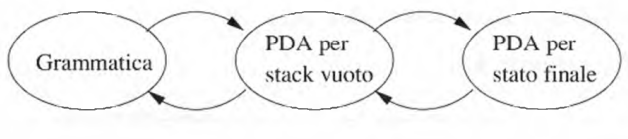
\includegraphics[width = 0.65\textwidth]{images/28.PNG}
\end{center}
Abbiamo già dimostrato che i linguaggi che vengono accettati da PDA per \textbf{stack vuoto} sono gli stessi accettati dai PDA \textbf{per stato finale}; quindi dimostriamo che le \textbf{grammatiche libere dal contesto} definiscono una classe di linguaggi equivalente alla classe dei linguaggi accettati dai PDA per stack vuoto.
\subsubsection{Da PDA a CFG}
Dato un PDA P che accetta per pila vuota, si costruisce una CFG in cui \textbf{le produzioni corrispondono al passaggio tra una configurazione alla successiva} in modo tale che le derivazioni della grammatica:
$$S \Rightarrow ... \Rightarrow w$$
Corrispondano ad un \textbf{passo di computazione dell'automa} e si arrivi a produrre la stringa $w \Leftrightarrow w \in N(P)$. 
\subsubsection{Da CFG a PDA che accetta per pila vuota}
Data una CFG $G = (V, T, Q, S)$ costruiamo il PDA $P$ che accetta il linguaggio $L(G)$ per pila vuota:
$$P = (\{q\}, T, V \cup T, \delta, q, S)$$
Con $\delta$ definita come segue:
\begin{itemize}
    \item $\forall A \in V, \delta(q, \varepsilon, A) = \{(q, \beta)|A \rightarrow \beta$ è una regola di produzione$\}$
    \item $\forall a \in T, \delta(q, a, a) = \{(q, \varepsilon)\}$
\end{itemize}
\begin{Osservazione}
    Per costruire un PDA per stati finali che accetta $L(G)$, lo si deve costruire a partire dall'automa a pila vuota.
\end{Osservazione}

\subsection{PDA Deterministici (DPDA)}
\begin{Definizione}
    Una PDA $P = (Q, \Sigma, \Gamma, \delta, q_0, z_0, F)$ è \textbf{determnistico} (cioè è un DPDA) se:
    \begin{enumerate}
        \item $|\delta(q, a, x)| \leq 1 \; \forall q \in Q, \; \forall a \in \Sigma \cup \{\varepsilon\}, 
        \; \forall x \in \Gamma$
        \item Se $|\delta(q, a, x)| \neq 0$ per qualche $a \in \Sigma$, allora $|\delta(q, \varepsilon, x)| = 0$
    \end{enumerate}
\end{Definizione}
\begin{Notazione}
    Quindi nei DPDA \textbf{le $\varepsilon$-transizioni esistono}, ma vengono semplicemente gestite in maniera diversa.
\end{Notazione}
\subsubsection{Linguaggi accettati dai DPDA}
I DPDA accettano una classe di linguaggi che si pone tra \textbf{i linguaggi context-free} e i \textbf{linguaggi regolari}. Iniziamo a dimostrare che i DPDA accettano tutti i linguaggi regolari:
\begin{Teorema}
    Se $L$ è un linguaggio regolare, allora $L = L(P)$ per un DPDA P
\end{Teorema}
\begin{Dimostrazione}
    Il DPDA è formato da un \textbf{controllo a stati finiti} e una pila. Se immaginiamo di \textbf{non utilizzare la pila}, cioè di leggere, togliere e rimettere $z_0$ costantemente, allora il DPDA sta a tutti gli effetti simulando un \textbf{DFA}.
\end{Dimostrazione}
Tuttavia, i DPDA \textbf{non accettano tutti i linguaggi context-free} ma solo una loro sottocategoria; cioè quei linguaggi che non hanno \textbf{grammatiche ambigue}. Inoltre i DPDA possono accettare per \textbf{pila vuota} solo se il linguaggio è \textbf{prefix-free}; diamo quindi qualche definizione:
\begin{Definizione}
    Una \textbf{prefissa} di una stringa $w \in L$ è una stringa $w'$ ottenuta togliendo 1 o più simboli dal fondo di $w$
\end{Definizione}
\begin{Definizione}
    Un linguaggio $L$ ha la \textbf{proprietà di prefisso}(cioè è \textbf{prefix-free}) se $\not\exists x, y \in L$ t.c. $x \neq y$ e $x$ è \textbf{prefissa} di $y$
\end{Definizione}
\begin{Osservazione}
    $\varepsilon$ è \textbf{prefissa di ogni stringa} di $L$, il linguaggio quindi non è prefix-free se $\varepsilon \in L$
\end{Osservazione}
Quindi possiamo enunciare il seguente teorema:
\begin{Teorema}
    Un linguaggio $L$ è $N(P)$ per un DPDA P $\Leftrightarrow$ $L$ ha la proprietà di prefisso (cioè è \textbf{prefix-free}); inoltre è $L(P')$ per un DPDA $P'$
\end{Teorema}
\begin{Dimostrazione}
    Immaginiamo di avere $L$ \textbf{NON} prefix-free, allora $\exists x,y \in L$ t.c. $x$ è \textbf{prefissa} di $y$. Allora, scomponiamo $y$ in $y = xw$ con $w \neq \varepsilon$ (poiché $x \neq y$). Assumiamo esista un DPDA $P$ t.c. $N(P) = L$. Se esso prende in input $x$, allora lo accetta, perché $x \in L$; quindi la pila è vuota. Tuttavia se gli passiamo $y = xw$, l'automa si ferma \textbf{prima che tutta la stringa venga consumata}, poiché \textbf{toglie $z_0$ dopo aver analizzato x}. Quindi è assurdo che esista un DPDA del genere.
\end{Dimostrazione}
Inoltre, possiamo enunciare i seguenti teoremi:
\begin{Teorema}
    Se $L$ è $N(P)$ per un DPDA $P$ allora $L$ ha una CFG non ambigua
\end{Teorema}
\begin{Teorema}
    Se $L$ è $L(P)$ per un DPDA $P$ allora $L$ ha una CFG non ambigua
\end{Teorema}
Riassumiamo ciò che abbiamo enunciato nel seguente schema:
\begin{center}
    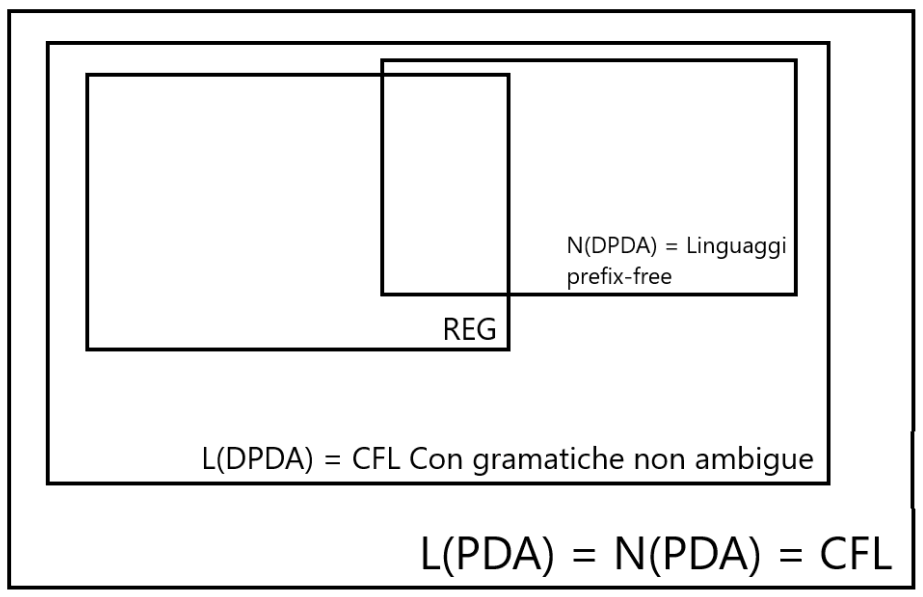
\includegraphics[width = 0.65\textwidth]{images/29.PNG}
\end{center}

\section{Macchine di Turing}
Alla fine dell' '800, inizio '900 ci fu il tentativo da parte di alcuni matematici, tra cui \textbf{Hilbert}, di formalizzare la matematica. Tra i problemi proposti da Hilbert vi era anche il cosidetto \textbf{Entscheidungsproblem} (problema della decisione), il quale chiedeve se esistesse una \textbf{procedura del tutto meccanica} in grado di stabilire, per ogni formula espressa nel linguaggio formale della logica del primo ordine, se tale formula è o meno un teorema della logica del primo ordine. È quindi possibile che i teoremi matematici siano \textbf{dimostrati da una macchina}? La risposta a questo problema fu data tramite i lavori di \textbf{Gödel}, \textbf{Turing} e \textbf{Church}. In particolare, Turing immaginò un "\textbf{matematico meccanico}" il cui "cervello" si trova in ogni istante in una configurazione diversa appartenente ad un insieme \textbf{finito di configurazioni}; esso dispone di un \textbf{nastro infinito} dove effettuare tutte le operazioni di lettura/scrittura e di una testina che punta, ad ogni istante, ad una cella del nastro. Ciò che quindi Turing immaginò è simile agli automi che abbiamo presentato finora; possiamo quindi immaginarne la funzione $\delta$ di transizione degli stati:
$$\delta(q, a) = (p, b, L)$$
$$\delta(q, B) = (...)$$
Il modello di calcolo teorizzato da Turing prende il nome di \textbf{macchina di Turing}(MdT), di cui adesso diamo una definizione formale dopo due brevi considerazioni:
\begin{Osservazione}
    Durante una computazione di una MdT, \textbf{la stringa non viene consumata}
\end{Osservazione}
\begin{Nota}
    Turing aveva inizialmente definito l'accettazione di una MdT di una stringa $w$ come l'evento in cui la macchina si ferma e non va in loop infinito. Per renderla più conforme alla teoria degli automi, si è preferito ridefinirla con \textbf{stati accentanti}.
\end{Nota}
\begin{Definizione}
    Una MdT è una settupla:
    $$M = (Q, \Sigma, \Gamma, \delta, q_0, B, F)$$
    Dove:
    \begin{itemize}
        \item $Q$ è l'insieme degli stati della macchina
        \item $\Sigma$ è l'alfabeto dei simboli di input
        \item $\Gamma$ è l'alfabeto dei simboli del nastro, inoltre $\Sigma \subseteq \Gamma$
        \item $\delta: Q \times \Gamma \rightarrow Q \times \Gamma \times \{L, R\}$ è la funzione di transizione degli stati. Essa prende in input lo stato attuale della macchine e il simbolo $a \in \Gamma$ che la testina di lettura/scrittura punta e restituisce una tripla $(p, \gamma, D)$ dove:
        \begin{itemize}
            \item $p \in Q$
            \item $\gamma \in \Gamma$ ed è il simbolo che andrà a sostituire $a$
            \item $D \in \{L, R\}$ che è la direzione in cui si muove la testina di lettura e scrittura. Essa si può quindi spostare di una cella a sinistra o a destra.
        \end{itemize}
        \begin{Osservazione}
            Così definita, \textbf{una computazione porta sempre allo spostamento della testina}
        \end{Osservazione}
        \item $q_0 \in Q$ è lo stato iniziale
        \item $B \in \Gamma \backslash \Sigma$ è il simbolo "Blank", cioè un simbolo che indica una cella \textbf{logicamente vuota}
        \item $F \subseteq Q$ sono gli stati finali
    \end{itemize}
\end{Definizione}
\begin{center}
    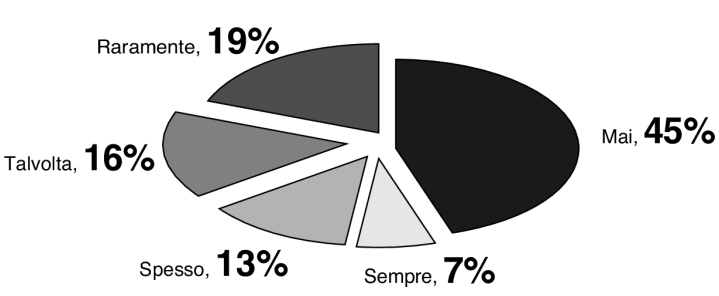
\includegraphics[width = 0.70\textwidth]{images/30.PNG}
\end{center}


\subsection{Configurazioni (o ID) di una MdT}
Un ID per una MdT ha la forma:
$$x_1x_2...x_{i-1}qx_ix_{i+1}...x_n$$
Supponiamo che $Q \cap \Sigma = \emptyset$. \newline
La testina è posizionata \textbf{sulla cella immediatamente a destra di q}. Prima di $x_1$ e dopo $x_n$ sono presenti solo simboli di blank.
\subsection{Passi di computazione di una MdT}
Descriviamo i passi di computazione di una MdT $M = (Q, \Sigma, \Gamma, \delta, q_0, B, F)$ mediante la notazione $\vdash_M$ già usata per i PDA. La relazione binaria $\vdash_M$ è assolutamente speculare a quella dei PDA, compreso il simbolo $\vdash^*_M$. Supponiamo che la M si trovi nella configurazione:
$$x_1x_2...x_{i-1}qx_ix_{i+1}...x_n$$
e che la funzione di transizione abbia il seguente caso: $$\delta(q_i, x_i) = (p, y, L)$$
Allora la nuova configurazione è:
$$x_1x_2...x_{i-2}px_{i-1}yx_{i+1}...x_n$$
Esistono due \textbf{casi particolari} per quanto riguarda uno spostamento a sinistra:
\begin{enumerate}
    \item Se $i = 1$ allora: $qx_1x_2...x_n \vdash_M pByx_2...x_n$
    \item Se $i = n$ e $y = B$, allora: $x_1x_2...x_{n-1}qx_n \vdash_M x_1x_2...x_{n-2}px_{n-1}$
\end{enumerate}
Quindi segnamo $B$ solo se viene puntato dalla testina della MdT.
Se invece la funzione di transizione avesse questo caso:
$$\delta(q_i, x_i) = (p, y, R)$$
allora la nuova configurazione è:
$$x_1x_2...x_{i-1}ypx_{i+1}...x_n$$
Esistono due \textbf{casi particolari} per quanto riguarda uno spostamento a destra:
\begin{enumerate}
    \item Se $i = n$, allora: $x_1x_2...qx_n \vdash_M x_1x_2...x_{n-1}ypB$
    \item Se $x = 1$ e $y = B$ allora: $qx_1x_2...x_n \vdash_M qx_2...x_n$
\end{enumerate}
\subsection{Diagramma di transizione per una MdT}
Possiamo costruire anche diagrammi di transizione per una MdT, utilizzando una notazione simile a quella dei PDA. Ogni nodo è uno \textbf{stato della MdT}. Un arco da uno stato $q$ a uno stato $p$ rappresenta una \textbf{possibile computazione} che porta la macchina dallo stato $q$ allo stato $p$ e ogni arco è etichettato da uno o più oggetti della forma $X/YD$ dove $X \in \Gamma$ è il simbolo presente sul nastro, $Y \in \Gamma$ è il simbolo che andrà a rimpiazzare $X$ e $D$ è la direzione in cui si sposta la testina. Uno stato accettante è contrassegnato da un doppio cerchio, mentre lo stato iniziale è contrassegnato da un arco entrante etichettato con \textbf{START}.
\begin{center}
    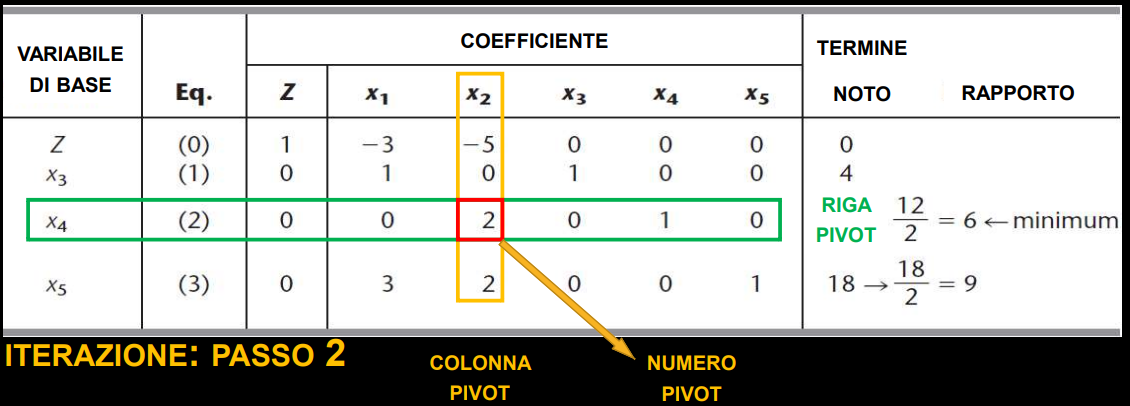
\includegraphics[width = 0.60\textwidth]{images/31.PNG}
\end{center}
\newpage
\subsection{Linguaggi accettati da una MdT: Linguaggi Ricorsivamente Enumerabili}
Sia $M = (Q, \Sigma, \Gamma, \delta, q_0, B, F)$ una MdT. Allora il linguaggio accettato da M è:
$$L(M) = \{w \in \Sigma^* | q_ow \vdash^*_M \alpha p \beta \; con \; p \in F \; e \; \alpha,\beta \in \Gamma^*\}$$
I linguaggi accettati dalle MdT si chiamano \textbf{linguaggi ricorsivamene enumerabili}, abbreviati in RE. Essi sono caratterizzabili in vari modi, tra i quali la seguente: "I linguaggi ricorsivamente enumerabili sono quei linguaggi per i quali esiste una procedura \textbf{"effettiva"}(quindi calcolabile) che stampa tutte le stringhe del linguaggio". Quindi $w \in L \Leftrightarrow$ appare in "output" dalla procedura, altrimenti \textbf{non posso affermare che non sia parte del linguaggio}. Inoltre la procedura potrebbe andare avanti all'infinito. Concludiamo presentando il seguente enunciato, tuttavia non in modo formale, chiamato \textbf{Tesi di Church-Turing}: "Tutto quello che è \textbf{computabile} con qualunque metodo di calcolo "ragionevole" è computabile da una MdT". Oltre alla MdT, esistono anche altri modelli di calcolo:
\begin{itemize}
    \item Macchine a registri/contatori
    \item Sistemi di riscrittura di Post: essi riscrivono pezzi di stringhe; la computazione avviene quindi su operazioni sulle stringhe
    \item ecc...
\end{itemize}
Tutti i modelli di calcolo classici sono \textbf{Turing-equivalenti}, cioè hanno la stessa potenza di una macchina di Turing. Esistono modelli più potenti? Si, per esempio modelli che effettuano computazioni sui \textbf{numeri reali} oppure le \textbf{macchine quantistiche}, le quali sono uguali alle MdT tranne per la loro capacità di \textbf{generare numeri randomici}.
\subsection{Estensioni della MdT}
Supponiamo di avere due modelli di calcolo $M_1$ e $M_2$. Se ogni computazione di $M_1$ è \textbf{simulabile} da $M_2$, allora \textbf{le macchine della classe $M_1$ NON potranno essere più potenti delle macchine della classe $M_2$}, cioè non possono riconoscere linguaggi "in più". Ciò si indica con:
$$M_1 \leq M_2$$
Se vale anche
$$M_2 \leq M_1$$
allora
$$M_1 = M_2$$
Vediamo ora delle estensioni equivalenti della MdT:
\subsubsection{MdT con la simbolo "Stay"}
Questa estensione modifica la funzione $\delta$ di transizione nel seguente modo:
$$\delta: Q \times \Gamma \rightarrow Q \times \Gamma \times \{L, S, R\}$$
S indica che la testina della MdT non si andrà a spostare dopo aver effettuato un passo di computazione. Questa MdT è facilmente simulabile da una MdT "standard" poiché ogni passo che indica alla MdT di non muovere la testina può essere simulato effettuando due mosse, una avanti e una indietro, dalla MdT standard.
\subsubsection{Macchine multinastro (con num. finito k di nastri)}
Una MdT multinastro si presenta nel seguente modo:
\begin{center}
    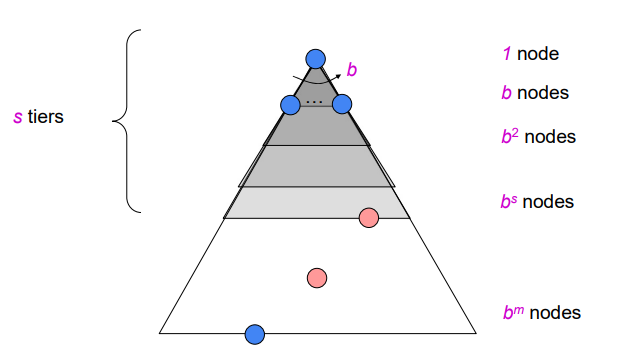
\includegraphics[width = 0.60\textwidth]{images/32.PNG}
\end{center}
quindi ha un controllo finito e un insieme finito di nastri. Ogni nastro è diviso in celle e ogni cella può contenere un simbolo dell'alfabeto finito di nastro; la quale definizione è identica a quella della MdT mononastro.  L'insieme degli stati comprende uno stato iniziale degli stati accettanti. All'inizio della computazione, valgono i seguenti criteri:
\begin{enumerate}
    \item L'input $w$, una sequenza finita di simboli, si trova sul 1° nastro
    \item Tutte le altre cellule di ogni nastro contengono $B$
    \item Il controllo si trova nello \textbf{stato iniziale}
    \item La testina del 1° nastro si trova all'estremo sinistro dell'input $w$
    \item Tutte le altre testine si trovano in posizione arbitraria; la loro posizione iniziale non importa poiché tutti i nastri eccetto il 1° partono "logicamente vuoti"
\end{enumerate}
Una mossa di una MdT multinastro dipende dallo stato del controllo finito e dai simboli $x_1, x_2, ..., x_k$ letti su ogni nastro. Quindi possiamo definire le operazioni eseguite dalla macchina come segue:
\begin{enumerate}
    \item Il controllo entra in un nuovo stato, che può coincidere con il corrente
    \item Su ogni cella della testina viene scritto un nuovo simbolo appartenente all'alfabeto finito dei simboli di nastro; il quale può coincidere con il corrente
    \item Ogni testina si muove a destra o a sinistra, indipendentemente dal movimento delle altre testine.
\end{enumerate}
Quindi una funzione $\delta$ ha questa forma:
$$\delta(q, x_1,x_2,...x_k) = (p, y_1, y_2, ..., y_k, D_1, D_2,...D_k)$$
Questa estensione è \textbf{Turing-equivalente}; infatti è banale mostrare come una MdT multinastro possa simulare una MdT mononastro; tuttavia, è più difficile mostrare la validità del seguente teorema:
\begin{Teorema}
    Ogni linguaggio accettato da una MdT multinastro è ricorsivamente enumerabile
\end{Teorema}
\begin{Dimostrazione}
    Possiamo simulare una MdT multinastro $M$ con una MdT mononastro $N$ definendo quest'ultima nel seguente modo:
    \begin{itemize}
        \item $x_1x_2...x_k$ diventa un nuovo \textbf{simbolo di nastro}
        \item Definisco quindi $N$ con un alfabeto di simboli di nastro che \textbf{contiene le $k$-uple} dell'alfabeto di simboli di nastro di $M$ (guardo quindi la funzione $\delta$)
        \item La riscrittura di una determinata $k$-upla sarà un altro simbolo che corrisponderà a $y_1y_2...y_k$
    \end{itemize}
    Questa dimostrazione è applicabile anche se le testine vanno in direzioni diverse.
\end{Dimostrazione}
\begin{Dimostrazione}[Libro]
    La dimostrazione è mostrata dalla seguente figura:
    \begin{center}
        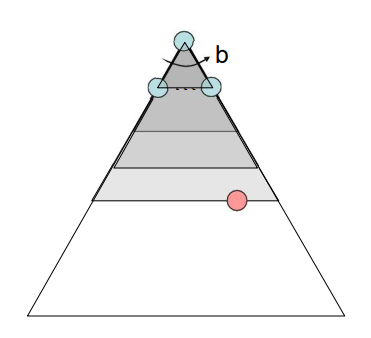
\includegraphics[width = 0.65\textwidth]{images/33.PNG}
    \end{center}
    Simuliamo una macchina multinastro $M$ attraverso una MdT mononastro $N$, il cui nastro è diviso in $2k$ \textbf{tracce}. Metà delle tracce sono usate per \textbf{replicare i nastri di M}; ognuna delle restanti ospita un \textbf{marcatore} che indica la posizione corrente della testina del corrispondente nastro di $M$. Chiamiamo $X$ questo marcatore (nella figura ipotizziamo $k = 2$). \newline
    Per simulare una mossa di $M$, la testina di $N$ deve visitare i $k$ marcatori. Per non smarrisi, $N$ deve tenere conto di \textbf{quanti marcatori stanno alla sinistra della testina in ogni istante}; il contatore è \textbf{conservato come componente del controllo finito di N}. Dopo aver visitato ogni marcatore e memorizzato, in una componente del controllo, il simbolo nella cella corrispondente, $N$ sa \textbf{quali sono i simboli che vengono guardati dalle testine di M}; inoltre $N$ conosce lo stato di $M$, memorizzato nel suo controllo. Perciò $N$ può dedurre la \textbf{prossima mossa di $M$}. \newline 
    Gli stati accettanti di $N$ sono quelli in cui è \textbf{registrato uno stato accettante di $M$}; in questo modo $N$ accetta solo quando $M$ accetta.
\end{Dimostrazione}
\subsubsection{MdT non deterministiche}
Una MdT non deterministica si distingue dalla MdT deterministica per la sua funzione $\delta$:
$$\delta: Q \times \Gamma \rightarrow 2^{(Q \times \Gamma \times \{L, R\})}$$
Ogni computazione quindi genera un \textbf{albero di computazione}, i cui nodi sono formati dalle \textbf{varie configurazioni che la MdT non determinstica assume nei vari casi della $\delta$}. \newline
Come facciamo a scoprire se c'è una configurazione accettante? Come per tutti i modelli di calcolo non deterministici che abbiamo visto, esistono due possibilità:
\begin{itemize}
    \item Ad ogni scelta non deterministica, la macchina "\textbf{si moltiplica}", tuttavia questo metodo è molto inefficiente
    \item Esiste \textbf{un oracolo} che guila la computazione. Possiamo quindi simulare questo oracolo?
\end{itemize}
Per gli NFA e $\varepsilon$-NFA era possibile convertendoli in DFA. I DPDA \textbf{riconscono meno linguaggi} dei PDA. Le MdT non deterministiche \textbf{sono Turing-equivalenti}, cioè riconoscono la stessa classe di linguaggi delle MdT deterministiche; infatti una MdT deterministica può essere vista come un \textbf{caso particolare di MdT non deterministica} con albero di computazione che presenta un solo nodo figlio per la radice e per tutti i suoi nodi intermedi e una sola foglia. Mostrare il contrario è più complesso:
\begin{Teorema}
    Se $M_N$ è una MdT non deterministica, esiste una MdT di Turing deterministica $M_D$ t.c. $L(M_N) = L(M_D)$
\end{Teorema}
\begin{Dimostrazione}
    Costruiamo la macchina multinastro $M_D$ come segue:
    \begin{center}
        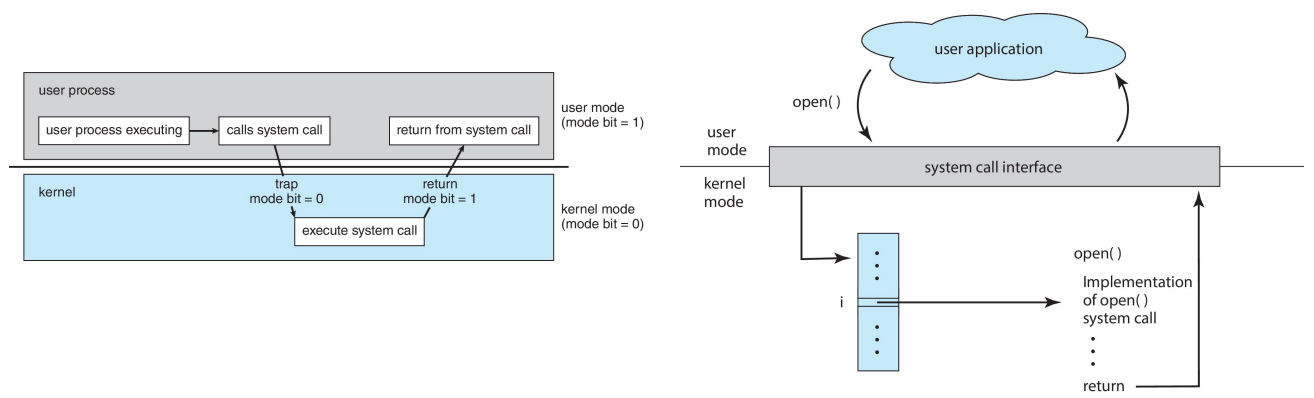
\includegraphics[width = 0.65\textwidth]{images/34.PNG}
    \end{center}
    La macchina multinastro $M_D$ ha un nastro contenente la \textbf{configurazione correntemente considerata} della macchina e un nastro "\textbf{coda}" in cui vengono immesse, ad ogni passo di computazione, le possibili prossime configurazioni da analizare. Il 2° nastro quindi funge da \textbf{coda} delle prossime configurazioni da analizzare e permette di analizzare l'albero di computazione \textbf{in ampiezza}. $M_D$ accetta solo se la configurazione (e quindi il nodo dell'albero di computazione) è accettante.
\end{Dimostrazione}
\subsection{Versioni ristrette delle MdT}
Una restrizione di una MdT può essere utile per rendere più semplice la dimostrazione di vari teoremi, purché essa rimanga comunque \textbf{Turing-equivalente}. Vediamo quindi ora delle restrizioni della MdT che comunque mantengono questa proprietà:
\subsubsection{MdT con nastri semi-finiti}
\begin{Teorema}
    Ogni linguaggio accetato da una MdT $M_2$ è accettato anche da una MdT $M_1$ con le seguenti restrizioni:
    \begin{enumerate}
        \item La testina di $M_1$ non va \textbf{mai a sinistra} della posizioni iniziale
        \item $M_1$ non scrive mai $B$ sul nastro
    \end{enumerate}
\end{Teorema}
\begin{Dimostrazione}
    È possibile simulare le MdT standard con questa restrizione. Per farlo costruiamo $M_1$ con un nastro infinito \textbf{solo a destra}. Per simulare una MdT standard, prendiamo tutto il nastro a sinistra della posizione iniziale e lo "giriamo" in modo da ottenere un nastro formato nel seguente modo:
    \begin{center}
        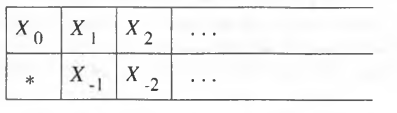
\includegraphics[width = 0.55\textwidth]{images/36.PNG}
    \end{center}
    Con $X_0, X_1, ...$ i simboli \textbf{a destra della pos. iniziale} e $X_{-1}, X_{-2}...$ i simboli \textbf{a sinistra della pos. iniziale}. Il simbolo $*$ indica la fine della traccia e impedisce che la testina "cada" accidentalmente fuori dal bordo del nastro. Definiamo quindi un nuovo alfabeto di simboli del nastro i cui simboli \textbf{rappresentano coppie dei simboli del nastro} formate prendendo i primi due simboli delle due "tracce" dall'altro verso il basso; considerando i due simboli come se fossero nella stessa cella. Il nuovo alfabeto sarà quindi formato da simboli rappresentanti coppie $(x_i, s)$. Per esempio, se una cella contiene la coppia $(a, b)$ possiamo assegnarle il simbolo $\alpha$; se per esempio voglio scrivere $c$ al posto di $b$, allora la coppia diverrà $(a, c)$ e possiamo assegnare a questa nuova configurazione il simbolo $\beta$. Quindi, ad esempio, un possibile nuovo alfabeto di nastro può avere questa forma:
    $$\Gamma_{M_1} = \{(a, *) = a_1, (b, c) = a_2, (i, b) = a_3 ...\}$$
    La 2° condizione si risolve sostituendo ogni scrittura di $B$ con un simbolo $B'$
\end{Dimostrazione}
\newpage
\subsubsection{Macchine multi-stack}
Consideriamo di avere un DPDA con $k$ pile formato nel seguente modo (nell'imagine si ipotizza $k = 3$):
\begin{center}
    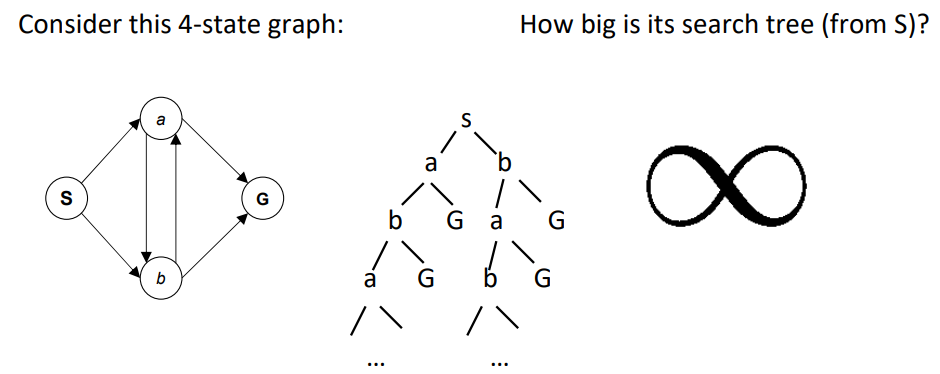
\includegraphics[width = 0.55\textwidth]{images/37.PNG}
\end{center}
Com'è fatta la $\delta$ di questo automa? Possiamo immaginarla come segue:
$$\delta(q, a(oppure \; \varepsilon), x_1, x_2, ..., x_k) = (p, \gamma_1, \gamma_2, ..., \gamma_k)$$
Cosa può fare questo tipo di automa? Vediamo il seguente teorema:
\begin{Teorema}
    Se un linguaggio $L$ è accettato da una MdT, allora $L$ è accettato anche da una macchina con almeno due stack.
\end{Teorema}
\begin{Dimostrazione}
    Si sfrutta il fatto che due stack possono \textbf{simulare il nastro di una MdT}: uno stack conserva ciò che sta a sinistra della testina e uno ciò che sta a destra della testina (sono escluse le infinte sequenze di $B$). In dettaglio, sia $L = L(M)$ per una MdT $M$ con un nastro. Descriviamo le operazioni che vengono compiute dalla macchina a due stack $S$:
    \begin{enumerate}
        \item $S$ comincia con i due stack "logicamente vuoti", quindi con solo il simbolo iniziale degli stack presente.
        \item $S$ legge la stringa $w$ di input e la \textbf{spinge} su una pila e poi lo travasa sull'altra: otteniamo una pila vuota e \textbf{una pila con in cima il carattere puntato dalla testina} della MdT all'inizio della computazione.
        \item L'automa simula un passo della MdT come segue:
        \begin{enumerate}
            \item $S$ conosce lo stato di $M$ poiché lo simula nel proprio controllo
            \item $S$ controlla cosa c'è in cima alla pila ed effettua un passo di computazione della MdT. In particolare:
            \begin{itemize}
                \item Se $M$ sostituisce $X$ con $Y$ e va a destra, allora $S$ pone $Y$ sul primo stack, a rappresentare che $Y$ ora è a sinistra della testina; $X$ viene tolto dal 2° stack di $S$. Ci sono due eccezioni:
                \begin{enumerate}
                    \item Se contiene solo l'indicatore di fondo, \textbf{il secondo stack non viene modificato}; poiché vuol dire che la testina si è spostata su un simbolo $B$
                    \item Se $Y = B$ e il 1° stack è vuoto, allora esso rimane vuoto, poiché a sinistra rimangono comunque solo blank.
                \end{enumerate}
                \item Se $M$ sostituisce $X$ con $Y$ e va a sinistra, $S$ toglie il simbolo in cima al primo stack (diciamo $Z$) e sostituisce $X$ con $ZY$ nel secondo stack. In questo modo si tiene conto del fatto che il simbolo che era immediatamente a sinistra della testina è ora sotto di essa. Si ha una sola eccezione quando $Z$ è il simbolo di fondo: $S$ deve allora porre $BY$ sul secondo stack senza togliere nulla dal primo.
            \end{itemize}
        \end{enumerate}
        \item $S$ accetta solo se si trova in uno stato di $M$ accettante.
    \end{enumerate}
\end{Dimostrazione}
\section{Computabilità}
\subsection{Indecidibilità}
Supponiamo esista un programma $H$ formato in questo modo:
\begin{center}
    \hspace{-2,9cm}
    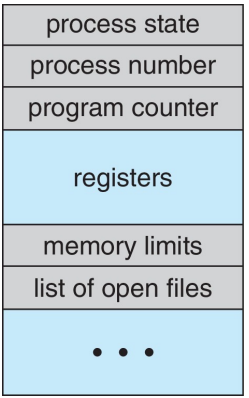
\includegraphics[width = 0.45\textwidth]{images/38.PNG}
\end{center}
Con $P$ un altro programma e $I$ un input da dare $P$. Quindi il programma $H$ cerca di \textbf{prevedere il comportamento di $P$} quando riceve un input $I$ e risponde "si" solo se i primi 11 caratteri stampati da $P$ con input $I$ sono "Ciao, mondo" . Se esiste però $H$ allora di sicuro esisterà anche un programma $H_1$ così costruito:
\begin{center}
    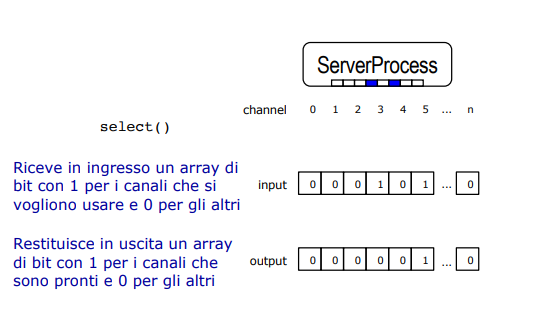
\includegraphics[width = 0.55\textwidth]{images/39.PNG}
\end{center}
Il quale è una semplice modifica di $H$; ma se esiste $H_1$ allora sicuramente esiste $H_2$ così costruito:
\begin{center}
    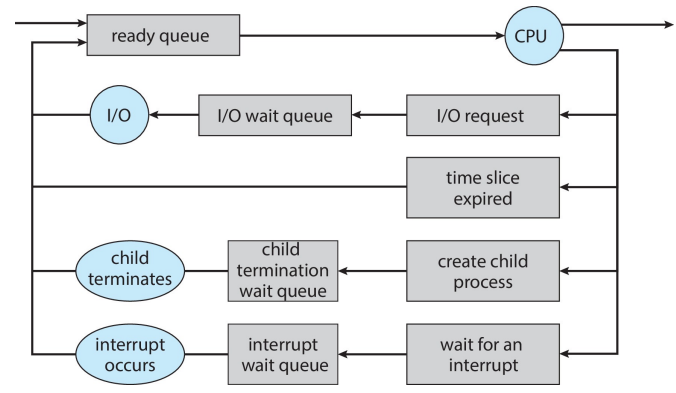
\includegraphics[width = 0.55\textwidth]{images/40.PNG}
\end{center}
Possiamo immaginare la struttura interna di $H_2$ così formata:
\begin{itemize}
    \item Una funzione "copy" che copia il programma di input e lo immagazina in $I$
    \item Una componente $H_1$ che prende in input $P$ e $I$
\end{itemize}
Poiché anche $H_2$ è un programma, allora possiamo fare:
\begin{center}
    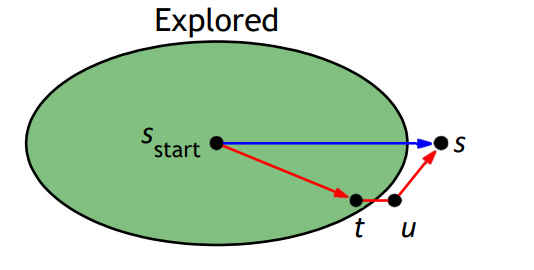
\includegraphics[width = 0.55\textwidth]{images/41.PNG}
\end{center}
Cosa quindi deve fare $H_2$? Deve analizzare se stesso e dare una risposta. Tuttavia, se stampa "si", allora \textbf{i primi 11 caratteri stampati non sono la stringa "Ciao, mondo"}. Allora dovrebbe stampare "Ciao, mondo", tuttavia allora \textbf{essi SONO gli 11 primi caratteri stampati dal programma}. Ci troviamo quindi davanti ad un \textbf{paradosso}, e per questo $H_2$ \textbf{non può esistere}. Ma allora neanche $H_1$ può esistere e allora neanche $H$ esiste.\newline
Quindi, in generale, \textbf{non esiste un programma che ne analizza un altro e ne prevede il comportamento}. Le "\textbf{prorpietà dinamiche}" (cioè del comportamento dei programmi) sono \textbf{indecidibili}. Esistono quindi dei problemi \textbf{indecidibili}.
\begin{Nota}
    Nella versione esposta, il problema contiene \textbf{autoreferenzialità}: $H_2$ analizza se stesso. Questa caratteristica è comune anche ad altri paradossi, come, per esempio, il \textbf{paradosso di Russel}
\end{Nota}
Un altro paradosso può essere:
\begin{center}
    "Questa frase è falsa"
\end{center}
Esaminiamo ora un programma $P$:
\begin{center}
    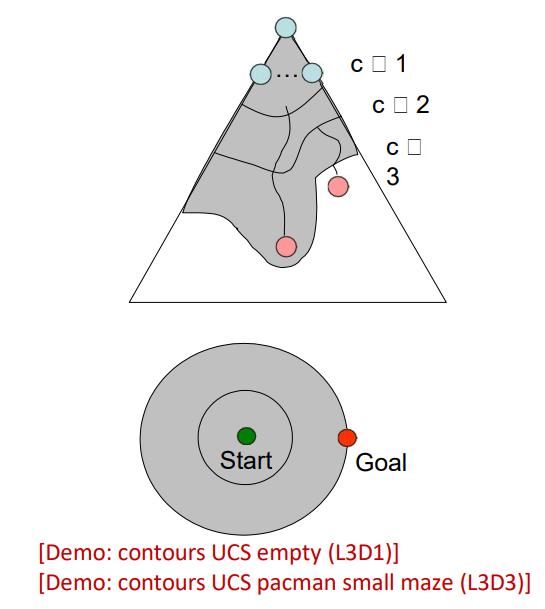
\includegraphics[width = 0.65\textwidth]{images/42.PNG}
\end{center}
Quindi che calcola $f_p: \mathbb{N} \rightarrow \mathbb{N}$. Quante sono queste funzioni? Se $|\mathbb{N}| = \aleph_0$ e $|\mathbb{R}| = \aleph_1$ allora le funzioni sono $|\mathbb{N}^\mathbb{N}| = \aleph_0^{\aleph_0}$. Quanti sono i programmi $P$? Poiché possiamo immaginarli come \textbf{sequenza di bit}, allora $|Progs| = \aleph_0 = |\mathbb{N}|$. Seppur \textbf{non sia mai stato dimostrato}, si pensa che:
$$\aleph_0 << \aleph_0^{\aleph_0}$$
Poiché le funzioni sono quindi \textbf{molte di più dei programmi}, allora \textbf{esistono funzioni non calcolabili} poiché non vi è un programma $P$ che le calcola. Queste funzioni sono \textbf{la maggioranza di tutte le funzioni esistenti}.
\subsection{Enumerazione delle stringhe binarie}
"Enumerare" significa dare una regola per il quale si possa elencare \textbf{in ordine} un insieme di oggetti. La regola che diamo per le stringhe binarie è la seguente: \newline
se $w \in \{0, 1\}^*$, consideriamo $1w$ come il numero intero $i$ (scritto in binario), e chiamo $w$ la $i$-esima stringa binaria e la indico con $w_i$. L'enumerazione quindi \textbf{elenca le stringhe in ordine di lunghezza}:
$$\varepsilon = 1\varepsilon = 1 \leftrightarrow w_1$$
$$0 = 10 = 2 \leftrightarrow w_2$$
$$1 = 11 = 3 \leftrightarrow w_3$$
$$00 = 100 = 4 \leftrightarrow w_4$$
$$...$$
La regola di enumerazione è quindi una \textbf{biezione}.
\subsubsection{Conversione da MdT a stringa binaria}
Codifichiamo una MdT come una \textbf{stringa binaria}: tuttavia, la vincoliamo per renderne la gestione più semplice: \newline
Consideriamo una MdT $M = (Q, \underbrace{\{0, 1\}}_\Sigma, \Gamma, \delta, q_1, B, \{q_2\})$ \newline
con:
\begin{itemize}
    \item $Q = \{q_1, q_2, ..., q_r\}$
    \item $\Gamma = \{X_1, X_2, ..., X_S\}$ dove $X_1 = 0, X_2 = 1, X_3 = B$
\end{itemize}
Le direzioni di spostamento non compaiono in questa definizione, ma le codifichiamo nella $\delta$ come:
$$L = D_1$$
$$L = D_2$$
Codifichiamo la $\delta$:
$$\delta(q_i, X_j) = (q_k, X_l, D_m)$$
Possiamo quindi codificare un generico case della $\delta$ usando questa notazione:
$$(i, j, k, l, m)$$
Con $i, j, k, l, m$ gli indici che appaiono nel generico caso della $\delta$ visto sopra. Rappresentiamo quindi la $5$-upla ottenuta in binario nel seguente modo:
$$(i, j, k, l, m) \rightarrow 0^i10^j10^k10^l10^m = C_1$$
(quindi, in effetti, gli indici sono \textbf{rappresentati in unario}). Cosa succede se abbiamo più casi della $\delta$ $C_1, C_2, ..., C_n$? Allora li rappresentiamo come segue:
$$C_111C_211..11C_N \in \{0, 1\}^*$$
Questa stringa \textbf{rappresenta tutta la $\delta$ della MdT} e \textbf{rappresenta una MdT}. Poiché abbiamo enumerato le stringhe binarie, in generale una stringa binaria \textbf{rappresenta un MdT}? In generale no; possiamo però risolvere questo problema nel seguente modo:
definisco una \textbf{macchina di default} che \textbf{contiene un solo stato e la sua $\delta$ è vuota}. La macchina quindi non effettua alcuna operazione e \textbf{non accetta mai}, quindi accetta il \textbf{linguaggio vuoto}. Ad ogni stringa che non può essere decodificata in una MdT ben formata associo questa macchina. \newline
Viceversa, ogni macchina di Turing è \textbf{rappresentabile come una stringa binaria}?
\begin{Osservazione}
    In generale una MdT può essere rappresentata da più stringhe binarie.
\end{Osservazione}
Effettuando questi accorgimenti, partendo dall'enumerazione delle stringhe binarie, si \textbf{costruisce l'enumerazione di tutte le possibili MdT}. \newline
Supponiamo di avere una macchina $M$ (scritta come visto prima) e una stringa binaria $w$. Se chiamo:
$$cod(M)$$
la stringa che rappresenta la MdT, allora posso costruire:
$$cod(M)111w$$
Ottenendo quindi una stringa binaria che \textbf{rappresenta la macchina e la sua stringa di input}; questo perché \textbf{$cod(M)$ non contiene mai 111}.
\subsection{Linguaggio di diagonalizzazione}
Indichiamo il \textbf{linguaggio di diagonalizzazione} con:
$$L_d = \{w_i \in \{0, 1\}^*|w_i \not\in L(M_i)\}$$
Le MdT sono in \textbf{corrispondenza biunivoca} con le stringhe binarie. Abbiamo quindi che la stringa $w_i$ rappresenta la \textbf{macchina di Turing $M_i$}(se non è una MdT valida, allora $M_i$ è la macchina di default). Costruiamo quindi la seguente tabella infinita:
\begin{center}
    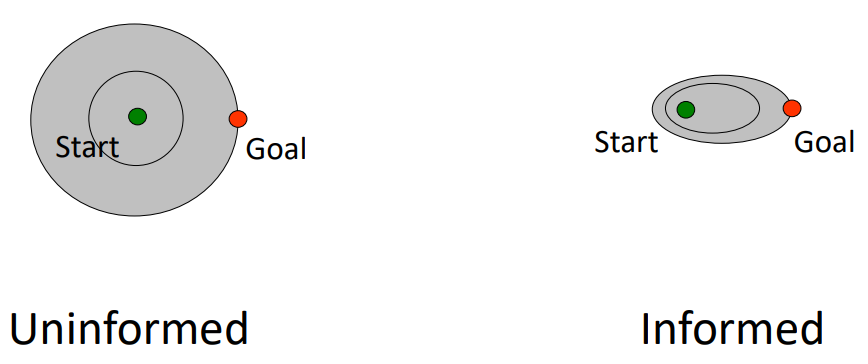
\includegraphics[width = 0.55\textwidth]{images/43.PNG}
\end{center}
Con le macchine $M_i$ associate alle righe della tabella e le stringhe di input $w_j$ associate alle colonne della tabella. Se in una cella $(i, j)$ è presente un $1$, allora la macchina $M_i$ accetta la stringa $w_j$, altrimenti la cella contiene 0 (non accetta/va in loop infinito).
\begin{Osservazione}
    Osservando tutte le colonne $j$ in cui vi è un 1 sulla riga $i$ si ha una \textbf{rappresentazione di $L(M_i)$}
\end{Osservazione}
\textbf{Perché si chiama "di diagonalizzazione"}? \newline
Consideriamo la diagonale principale, cioè quindi consideriamo i valori della tabella per cui $i = j$. Consideriamo il \textbf{complemento} della stringa formata dai valori della diagonale:
$$L_d = (1,0,0,0...)$$
$L_d$ è il \textbf{vettore che rappresenta il linguaggio $L_d$} poiché contiene un $1$ per tutte le $w_i \not\in L(M_i)$. Quindi, nella matrice costruita, si ha $1$ nella posizione $(i, i) \Leftrightarrow$ \textbf{la macchina di Turing $M_i$ accetta se stessa come input}. \newline
Il linguaggio di diagonalizzazione è quindi \textbf{l'insieme di tutte le stringhe binarie che non vengono accettate dalle macchine di Turing rappresentate da quelle stringhe}. È quindi formato da tutte le stringhe binarie che \textbf{codificano MdT che non accettano se stesse}. Il vettore riportato sopra è quindi \textbf{il vettore caratteristico del linguaggio diagonale}, poiché contiene un $1$ in ogni posizione dove $w_i \not\in L(M_i)$. \newline \newline
\textbf{Questo linguaggio è Ricorsivamente Enumerabile}?
\begin{Teorema}
    $L_d$ \textbf{NON} è un linguaggio ricorsivamente enumerabile. Cioè non esiste nessuna MdT che lo accetta.
\end{Teorema}
\begin{Dimostrazione}
    Abbiamo detto che, per definizione, un linguaggio RE è un linguaggio \textbf{accettato da una MdT}. Ogni riga della tabella costruita sopra \textbf{contiene il vettore caratteristico del linguaggio accettato dalla MdT corrispondente}. Tuttavia, $L_d$ non può comparire nella tabella, poiché ogni suo elemento $x_i$ è \textbf{complemento} dell'elemento $k_{i, i}$ della tabella. Quindi $L_d$ \textbf{non è ricorsivamente enumerabile}
\end{Dimostrazione}
\begin{Dimostrazione}[Libro]
    Supponiamo $L_d = L(M)$ per una MdT $M$. Poiché $L_d$ è un linguaggio sull'alfabeto $\{0, 1\}$, $M$ rientra nell'elenco delle MdT che abbiamo costruito, dato che questo elenco include tutte le MdT con alfabeto di input $\{0, 1\}$. Di conseguenza, esiste almeno un codice per $M$, diciamo $i$, cioè $M = M_i$. Chiediamoci ora se $w_i \in L_d$:
    \begin{itemize}
        \item Se $w_i \in L_d$, allora $M_i$ accetta $w_i$. Pertanto, per definizione di $L_d$, $w_i$ non è in $L_d$, poiché esso contiene solamente le stringhe $w_j$ tali che $w_j \not\in L(M_j)$
        \item Se $w_i \not\in L_d$, allora $M_i$ non accetta $w_i$. Pertanto, per definizione di $L_d$, $w_i$ appartiene a $L_d$.
    \end{itemize}
    Poiché $w_i$ può non essere ed essere in $L_d$, abbiamo una contraddizione, quindi una macchina $M$ che accetta $L_d$ non può esistere. Quindi $L_d \not\in RE$
\end{Dimostrazione}
\subsection{Classificazione dei linguaggi}
Presentiamo il seguente schema:
\begin{center}
    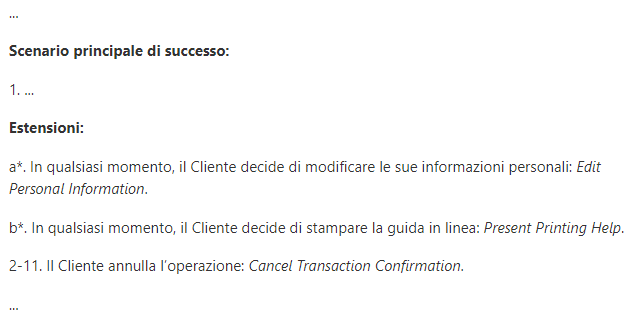
\includegraphics[width = 0.65\textwidth]{images/44.PNG}
\end{center}
E presentiamo la nuova classe dei linguaggi ricorsivi:
\subsubsection{Linguaggi ricorsivi}
Supponiamo di avere un linguaggio $L \in RE \backslash RIC$. Allora esiste una MdT $M_L$ t.c. $L = L(M_L)$. Per una stringa di input $w \in \Sigma^*$, la macchina $M_L$ può accettare e fermarsi, non accettare e fermarsi oppure \textbf{andare in loop infinito}. Capire se $M_L$ non accetta oppure va in loop infinito è un \textbf{problema indecidibile}. \newline
Supponiamo allora di avere $L_1 \in RIC$, allora esiste una MdT $M_{L_1}$ t.c. $L = L(M_{L_1})$. In particolare:
\begin{Definizione}
    Diremo \textbf{ricorsivo} (RIC) un linguaggio $L$ se $L = L(M)$ per una MdT $M$ t.c.:
    \begin{enumerate}
        \item $se \; w \in L$, allora la MdT accetta (e dunque si arresta)
        \item $se  \; w \not\in L$ allora la MdT rifiuta e si arresta.
    \end{enumerate}
\end{Definizione}
I linguaggi ricorsivi sono i linguaggi più vicini alla nozione di algoritmo. In particolare i linguaggi ricorsivi si dicono \textbf{decidibili}, quelli RE ma non RIC si dicono \textbf{semi-decidibili} e quelli non RE si dicono \textbf{indecidibili}.
\subsection{Complemento di un linguaggio}
\subsubsection{Linguaggi ricorsivi}
Prendiamo $L_2 \in RIC$. Il complemento di $L_2$:
$$\overline{L_2} = \{w \in \Sigma^* \backslash L_2\}$$
Inoltre:
\begin{Teorema}
    Se $L \in RIC$ allora $\overline{L} \in RIC$
\end{Teorema}
\begin{Dimostrazione}
    Il teorema si dimostra considerando la macchina $M_L$, che accetta $L$ e costruendo, basandosi su di essa, la macchina $M_{\overline{L}}$ che accetta il linguaggio $\overline{L}$. In particolare, si scambiano \textbf{gli stati finali con quelli non finali}. La nuova macchina costruita accetta il linguaggio $M_{\overline{L}}$ e si fermerà \textbf{sempre}, quindi $M_{\overline{L}} \in RIC$
\end{Dimostrazione}
\subsubsection{Ricorsivamente enumerabili ma non ricorsivi}
Prendiamo $L_1 \in RE \backslash RIC$. Consideriamo il complemento:
$$\overline{L_1} = \{w \in \Sigma^* \backslash L_1\}$$
Allora $\overline{L_1} \in RE \backslash RIC$? Se fosse così, allora posso costruire una MdT $M_{\overline{L_1}}$ tale che accetti $\overline{L_1}$ ma che abbia la possiblità \textbf{di non accettare o di andare in loop infinito}. Ma allora \textbf{posso costruire una MdT che simula} sia la macchina $M_{\overline{L_1}}$ sia la macchina $M_{L_1}$ che accetta il linguaggio $L_1$. In particolare, la nuova macchina simula un passo di computazione delle 2 macchine \textbf{in maniera alternata}(cioè prima fa un passo di $M_{L_1}$ poi un passo di $M_{\overline{L_1}}$ e così via). Chiamo questa macchina $M_L$. Tuttavia, questa macchina \textbf{non presenta il rischio di non arrestarsi mai}, poiché simula le 2 macchine in maniera alternata e una delle 2 prima o poi si fermerà (una qualsiasi stringa $w$ appartiene o a $L_1$ oppure a $\overline{L_1}$, non vi è una terza opzione); quindi $M_L$ è una \textbf{macchina che si ferma sempre} e che accetta $L_1$, quindi $L_1 \in RIC$, quindi, per il \textbf{teorema 8.5.1}, anche $\overline{L_1} \in RIC$. \newline Quindi \textbf{non è possibile} che $L_1 \in RE \backslash RIC$ e $\overline{L_1} \in RE \backslash RIC$, poiché altrimenti sarebbero entrambi ricorsivi. Ma allora $\overline{L_1}$ a che famiglia appartiene? $\overline{L_1} \in non \; RE$, quindi è \textbf{indecidibile}.
\section{Macchine di Turing universali e altre definizioni}
Poiché possiamo codificare una MdT in stringa binaria, allora possiamo \textbf{costruire una macchina di Turing} che prende in input la descrizione (stringa) di un'altra MdT e una stringa di input per quella macchina e \textbf{simuli} la macchina in input sulla stringa in input. Questa macchina quindi può accettare la stringa in input, rifiutare la stringa in input oppure \textbf{andare in loop infinito}. Il linguaggio accettato da questa macchina è chiamatao \textbf{linguaggio universale $L_U$}, che possiamo definire come:
$$L_U = \{cod(M)111w \in \{0, 1\}^*|w \in L(M)\}$$
Per il comportamento della macchina universale si evince che:
$$L_U \in RE \backslash RIC$$
Quindi $\overline{L_U} \in non \; RE$
Presentiamo quindi la struttura e il comportamento della macchina di Turing universale $U$:
\begin{enumerate}
    \item All'inizio della computazione, 1° testina è posizionata sul 1° bit di $cod(M)$ e tutti gli altri nastri sono riempiti di $B$
    \item Un passo di computazione \textbf{utilizza il 2° nastro} come se fosse il nastro della macchina simulata; quindi cerca $w$ nel 1°nastro e la \textbf{copia} nel 2°, quindi torna indietro con la 2° testina, posizionandola sul 1° bit di $w$.
    \item Dopodiché, per definizione, scrive lo stato iniziale $q_1$ sul 3° nastro.
    \item La macchina universale effettua una \textbf{scansione} per verificare che \textbf{vi sia un caso della $\delta$ associato al 1° bit di $w$ e a $q_1$} e, in caso esista, lo \textbf{simula} andando a modificare $w$, lo stato della macchina simulata $M$ e la posizione della testina del 2°nastro. Questo passo si itera fino a quando la macchina si ferma e accetta, si ferma e non accetta oppure \textbf{va in loop infinito}. Quindi simula \textbf{perfettamente $M$}
\end{enumerate}
\begin{center}
    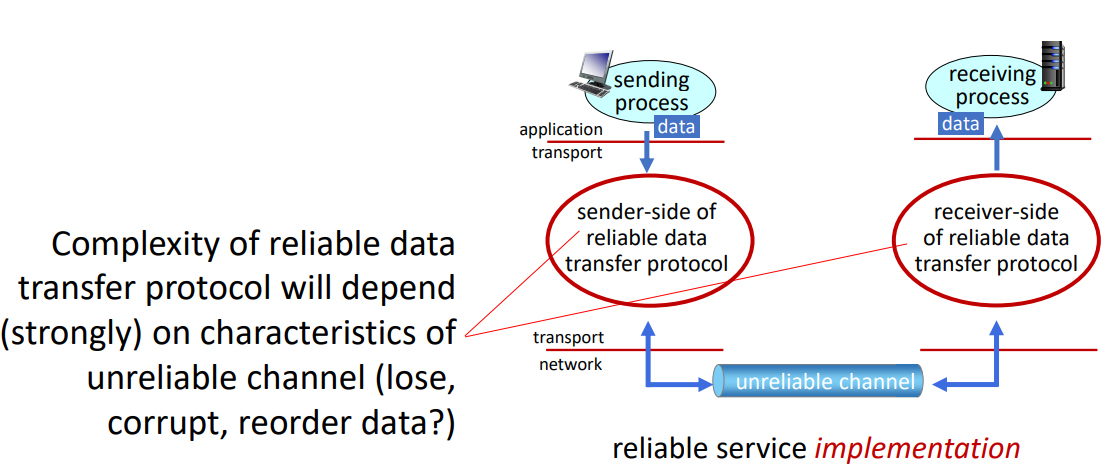
\includegraphics[width = 1\textwidth]{images/45.PNG}
\end{center}
La macchina universale accetta \textbf{il linguaggio universale}.
\subsection{Macchine di Turing che accettano il linguaggio vuoto}
Consideriamo un alfabeto $\Sigma = \{0, 1\}$, un linguaggio è quindi $L \subseteq \Sigma^*$. Prendiamo ora \textbf{l'enumerazione delle macchine di Turing}:
$$M_1 \leftrightarrow w_1$$
$$M_2 \leftrightarrow w_2$$
$$M_3 \leftrightarrow w_3$$
$$M_4 \leftrightarrow w_4$$
$$...$$
Quindi $cod(M_i) = w_i$. Formiamo un linguaggio $L = \{w_2, w_5, ..., w_10, ...\} \subseteq \{0, 1\}^* = \{M_2, M_5, ..., M_10, ...\}$. Allora possiamo formare un linguaggio nel modo seguente:
$$L_E = \{M|L(M) = \emptyset\}$$
Cioè l'insieme delle MdT che \textbf{accettano il linguaggio vuoto}. Considero anche il suo complemento:
$$L_{NE} = \{M|L(M) \neq \emptyset\}$$
In particolare, $L_E$ contiene \textbf{tutte le copie della macchina di default}. Dove si "trovano" questi linguaggi?
\begin{Teorema}
    Il linguaggio $L_{NE} \in RE$
\end{Teorema}
\begin{Teorema}
    Il linguaggio $L_{NE} \not \in RIC$
\end{Teorema}
\begin{Teorema}
    Il linguaggio $L_E \not\in RE$
\end{Teorema}
\subsection{Proprietà di un linguaggio RE e teorema di Rice}
\begin{Definizione}
    Una proprietà dei linguaggi RE è un insieme di linguaggi RE
\end{Definizione}
\begin{Definizione}
    Una proprietà dei linguaggi RE è \textbf{banale} se è l'insieme vuoto oppure se è l'insieme che contiene tutti i linguaggi RE
\end{Definizione}
\begin{Definizione}
    Una proprietà dei linguaggi RE è \textbf{non banale} se non è banale
\end{Definizione}
Sappiamo che $L \in RE \Leftrightarrow \exists M \; t.c. \; L = L(M)$. Tuttavia, non possiamo riconoscere un insieme di linguaggi come i linguaggi stessi. La ragione è che il tipico linguaggio è \textbf{infinito} e quindi non può essere espresso con una stringa di lunghezza finita che possa essere l'input di una MdT. Dobbiamo piuttosto \textbf{riconoscere le MdT che accettano quei linguaggi}: il codice di una MdT è \textbf{finito} anche se il linguaggio che accetta è infinito. Di conseguenza, se $P$ è una proprietà dei linguaggi RE, il linguaggio $L_P$ è \textbf{l'insieme dei codici delle MdT $M_i$ tali che $L(M_i) \in P$}. Quando quindi parliamo di \textbf{decidibilità di una proprietà $P$}, intendiamo quindi la decidibilità di $L_P$. Quindi enunciamo il seguente teorema:
\begin{Teorema}[Teorema di Rice]
Ogni proprietà non banale dei linguaggi RE è \textbf{indecidibile}
\end{Teorema}
\section{Ringraziamenti e note}
Si ringraziano tutte le persone che hanno contribuito a correggere e stilare questo \newline documento.
\end{document}
